\documentclass[../main]{subfiles}

\ifSubfilesClassLoaded{
    \addbibresource{../Biblio/biblio.bib}
    \dominitoc
    \tableofcontentsfile
    \pagenumbering{arabic}
    \setcounter{page}{1}
}{}

\begin{document}
\graphicspath{{./figures},{02-Architectures/figures}}
\chapter{Architectures de cartes auto-organisatrices}\label{chap:architectures}
\minitoc

\section{Introduction}

Les travaux que nous présentons dans cette thèse se concentrent sur la création d'une architecture non hiérarchique modulaire de cartes auto-organisatrices (SOM).
Les cartes auto-organisatrices et notamment le modèle de Kohonen sont principalement utilisées en tant qu'algorithme d'apprentissage non supervisé appliqué à des tâches de réduction de dimension, de visualisation de données ou de classification.
D'une part, de nombreux travaux étudient l'utilisation de plusieurs cartes collaborant entre elles sur différentes applications, en général afin d'améliorer les performances de classification ou de regroupement de données d'une carte auto-organisatrice classique. Ces travaux se retrouvent sous le terme de SOM hiérarchiques, SOM multi-couches, ou \emph{Deep SOM}.
Cependant, peu de travaux ont exploré l'aspect topologiquement ordonné et la simplicité des règles de mise à jour d'une carte pour les assembler en architectures modulaires comportant des rétroactions, c'est-à-dire des architectures non-hiérarchiques.

L'étude d'une architecture non hiérarchique de SOM est motivée par leur inspiration biologique. Le cortex faisant apparaître des aires interagissant entre elles avec des boucles de rétroaction, la création d'une architecture non hiérarchique de cartes s'inscrit dans la continuité de cette inspiration biologique.
Ensuite, l'étude des systèmes biologiques et la robotique peuvent être liées~: la biologie sert d'inspiration à la robotique, que ce soit pour le mouvement d'un bras ou la prise de décision, et la robotique permet de tester des théories cherchant à modéliser des comportements biologiques \parencite{Oudeyer2010OnTI}.
Aussi, les architectures de cartes bio-inspirées que nous avons relevées dans la littérature se définissent des domaines soit de l'apprentissage automatique, soit des neurosciences computationnelles ou de l'apprentissage incarné en robotique (\emph{Embodied intelligence}) \parencite{Smith2005TheDO,cangelosi_embodied_2015}, à la frontière entre étude de la biologie et apprentissage automatique.

Nous nous intéressons dans ce chapitre à un ensemble de travaux définissant des architectures de cartes auto-organisatrices, en s'intéressant aux différentes formes de modularité qu'elles implémentent.
La notion d'architecture modulaire de cartes est d'ailleurs résumée par Kohonen dès 1995~:
\begin{quote}
Un objectif à long terme de l'auto-organisation est de créer des systèmes autonomes dont les éléments se contrôlent mutuellement et apprennent les uns des autres. De tels éléments de contrôle peuvent être implémentés par des SOMs spécifiques~; le problème principal est alors l'interface, en particulier la mise à l'échelle automatique des signaux d'interconnexion entre les modules et la collecte de signaux pertinents comme interface entre les modules. Nous laisserons cette idée aux recherches futures.
Traduit de \cite{Kohonen1995SelfOrganizingM}
\end{quote}

L'objectif de nos travaux est ainsi de proposer un modèle de carte qui puisse être utilisée en tant que module, de définir l'interface entre les modules afin de créer une architecture, puis de comprendre les comportements de calcul qui émergent de l'association des modules.
Nous présentons dans ce chapitre le modèle général d'une carte de Kohonen et ses comportements fondamentaux, puis répertorions les différents types de structures se présentant comme des architectures de cartes. Nous pourrons ainsi définir en pratique la notion d'architecture modulaire et comment se placent nos travaux dans cette taxonomie.

\section{Les cartes auto-organisatrices de Kohonen comme modules d'une architecture}\label{sec:som001}

Le modèle de cartes auto-organisatrices a été initialement développé par Kohonen \parencite{Kohonen1982}~; nous utiliserons les termes cartes de Kohonen et SOM de façon équivalente pour désigner ce modèle initial.
De nombreux modèles ont ensuite été dérivés à partir de ce dernier, pour diverses applications.
Nous présentons dans cette section le modèle initial de carte de Kohonen et introduisons les notations que nous utiliserons dans ce manuscrit.

\subsection{Description du modèle de carte auto-organisatrice de Kohonen}\label{sec:modele_som}

\begin{figure}
    \centering
    \includegraphics[width=0.8\textwidth]{soms_topologies}
    \caption{Exemples de topologies utilisées pour des SOM. Les SOM en deux dimensions sont les plus communément utilisées dans la littérature, sous forme d'une grille ou d'une grille hexagonale. Les SOMs une dimension sont parfois utilisées. Cette topologie définit un voisinage entre les n\oe{}uds~: par exemple, le voisinage à une distance de une unité du n\oe{}uds coloré en rouge sont les n\oe{}uds colorés en orange~; les n\oe{}uds colorés en jaune sont à une distance de deux unités.
    \label{fig:topo}}
    \end{figure}

\begin{figure}
    \centering
    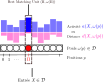
\includegraphics{SOM.pdf}
    \caption{\'Elements principaux composant une carte de Kohonen~: une carte possède un ensemble d'unités de poids $\omega$, indexées par une position $p$. En présence d'une entrée $X$, une activité $a$ ou une distance $d$ est calculée pour chaque unité par rapport à l'entrée. La \emph{Best Matching Unit}, abrégée en BMU, est calculée comme l'unité d'activité maximale sur les positions (ou de distance minimale). Sa position est notée $\bmu$ et son poids est $\w(\bmu)$.\label{fig:SOM}}
    \end{figure}

Une carte de Kohonen est un algorithme de quantification vectorielle. 
Les algorithmes de quantification vectorielle cherchent à représenter un ensemble de données d'entrées issues d'un espace $\mathcal{D}$ en un nombre fini de vecteurs de l'espace d'entrée, les prototypes.
Une carte auto-organisatrice ajoute une topologie sur laquelle s'appuie cette représentation. Les prototypes $\w$ sont alors positionnés sur les n\oe{}uds d'un graphe, et indexés par une position $p$. 
Ce graphe se présente comme une grille de faible dimension, en général une grille 2D, définissant une correspondance directe entre la dimension de la carte les positions $p$ des n\oe{}uds.
(\emph{mapping}). Des exemples de topologies de SOM 1D et 2D sont par exemple illustrées en figure~\ref{fig:topo}.

Avant apprentissage, ces prototypes sont initialisés aléatoirement dans l'espace d'entrée.
Une itération d'apprentissage comporte ensuite trois étapes~:
\begin{enumerate}
\item Une entrée $\inpx$ est présentée à toute la carte.
\item Le n\oe{}ud ayant le prototype le plus proche de $\inpx$ selon une distance $d(\w, \inpx)$ est choisi comme \emph{Best Matching Unit} (BMU) de la carte. Son indice est noté $\bmu$. \begin{equation}
    \bmu = \argmin\limits_p d(\w(p),\inpx)
\end{equation}

Ce calcul de distances, utilisé dans la version originale de SOM, est remplacé dans d'autres modèles de cartes par le calcul d'une \emph{activation} $a(p, \w, \inpx)$ liant les poids des n\oe{}uds et les entrées.
La BMU est alors l'unité située au maximum de l'activation. Cette étape est résumée en figure~\ref{fig:SOM}.
\item Le prototype du BMU $\w(\bmu)$ ainsi que les prototypes des n\oe{}uds voisins sont déplacés vers l'entrée $\inpx$. Le déplacement est pondéré par leur degré de proximité au BMU par une fonction de voisinage $H(p,\bmu)$
\begin{equation} \forall p, \:\w(p) \leftarrow \w(p) + \alpha H(\bmu,p) \left( \inpx - \w(p)\right) \end{equation}
$H$ définit l'amplitude de modification de chaque prototype $\w(p)$, en modulant le taux d'apprentissage $\alpha$ par $H(p,\bmu)$. $H$ est maximale à la position du BMU et décroissante autour de cette position, de sorte que les prototypes des n\oe{}uds les plus proches de $\bmu$ soient les plus influencés par le déplacement. Il s'agira par exemple d'une fonction rectangulaire, triangle ou gaussienne, illustrées en figure~\ref{fig:h}.
\end{enumerate}

\begin{figure}
     \centering
     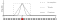
\includegraphics[width=0.6\textwidth]{voisinage.pdf}
     \caption{Exemples de fonctions de voisinage (Rectanglulaire, Triangle ou Gaussienne), centrées sur le BMU $\bmu$, couramment utilisées sur une carte, ici en une dimension.\label{fig:h}}
\end{figure}

L'algorithme de mise à jour des cartes de Kohonen repose à la fois sur un mécanisme de compétition par la sélection de la BMU de la carte et un processus de coopération avec le déplacement des unités voisines de la BMU, aussi nommé \og Winner Take Most \fg{}.
Le processus de mise à jour des poids d'une carte de Kohonen se traduit par un dépliement de la carte dans l'espace d'entrée. On parlera donc aussi de \emph{dépliement} d'une carte lorsque qu'on parle d'apprentissage. Ce dépliement est représenté en figure \ref{fig:som1d} pour des exemples de cartes en une et deux dimensions, se dépliant sur des données en deux dimensions.
\`A la fin de l'apprentissage, la carte conserve la structure topologique des entrées~:
\begin{itemize}
\item Elle conserve les distances~: deux prototypes ayant une distance proche dans la carte seront également proches selon la distance définie dans l'espace d'entrée. On observe alors une continuité des valeurs des poids au sein de la carte.
\item Elle conserve les densités. Une zone dense de l'espace d'entrée $\mathcal{D}$ sera représentée par plus de prototypes au sein de la carte, qu'une zone de faible densité.
\end{itemize}

% Par exemple, la figure \ref{fig:digits} représente le dépliement d'une carte sur des imagettes de taille $28\times 28$. Par son aspect ordonné, une carte est une représentation en dimension 2 d'un espace d'entrée de grande dimension.

\begin{figure}
\begin{minipage}{0.5\textwidth}
\centering
\includegraphics[width=\textwidth]{som2d}
% \caption{Dépliement d'une SOM 2D sur des données dans le plan $[0,1]^2$ au cours des itérations d'apprentissage \parencite{Kohonen1995SelfOrganizingM} \label{fig:som2d}}
%\end{figure} 
\end{minipage}
\begin{minipage}{0.5\textwidth}
\centering
\includegraphics[width=\textwidth]{som1d}
\end{minipage}
\caption{Exemples de dépliement d'une SOM 2D sur des données dans un carré (à gauche) et d'une SOM 1D sur des données dans un triangle 2D (à droite) au cours des itérations d'apprentissage \parencite{Kohonen1995SelfOrganizingM}\label{fig:som1d}}
\end{figure}
    
\subsection{Interprétation d'une carte de Kohonen comme un algorithme d'apprentissage de représentation}

La carte de Kohonen se distingue d'autres algorithmes de quantification vectorielle par la topologie introduite par la carte dans l'ensemble des prototypes.
Par sa topologie, une carte de Kohonen permet d'extraire une \emph{représentation} de l'espace d'entrée en faible dimension~: une carte 2D extrait ainsi une paramétrisation en 2D de l'espace des entrées $\mathcal{D}$.
Chaque élément de l'espace d'entrée peut être représentée par un vecteur 1D ou 2D, qui est la position du Best Matching Unit correspondant dans la carte.

En théorie, les cartes peuvent être en une dimension (ligne), deux dimensions (grilles), ou de dimensions plus grandes. Les cartes peuvent aussi être des graphes de forme plus variable. 
En pratique, les grilles en deux dimensions sont les supports les plus couramment utilisés. Les cartes de dimensions supérieures sont très rarement utilisées dans la littérature. 
Le coût de l'algorithme d'apprentissage dépend en effet du nombre de n\oe{}uds, et celui-ci augmente exponentiellement lorsqu'on augmente la dimension d'une carte de Kohonen.

Les cartes une dimension sont quant à elles plus limitées que les cartes 2D en termes de représentation des données et sont donc rarement utilisées en pratique ou sur des applications dérivées, par exemple pour de la planification de chemin \parencite{FrezzaBuet2020SelforganizingMI}.
Cependant, elles se prêtent mieux à la représentation graphique et au développement de nouveaux modèles de SOM que les cartes 2D.
Les travaux conduits en \cite{Cottrell1998TheoreticalAO,fort_soms_2006} apportent par exemple une formalisation mathématique de l'algorithme de Kohonen et prouvent la convergence de cartes une dimension. Les auteurs se heurtent cependant à la preuve de convergence pour des cartes en deux dimensions. 
Les processus intervenant dans des cartes 1D sont donc mathématiquement difficiles à formaliser, et cette difficulté augmente avec les dimensions de la carte.

Si les cartes de forme autre que des grilles 1D ou 2D sont moins couramment utilisées, elles peuvent présenter des avantages. Ainsi, des cartes structurées en arbre telles que développées en~\cite{koikkalainen_self-organizing_1990} permettent une recherche de BMU plus rapide au sein de la carte, adaptées à des données d'entrée présentant une structure hiérarchique. Certains modèles construisent une carte de Kohonen incrémentale en ajoutant des n\oe{}uds au fur et à mesure de l'apprentissage, générant une carte de Kohonen sous forme d'un graphe construit par l'algorithme, par exemple en~\cite{Fritzke1995GrowingG, alahakoon_dynamic_2000, yamaguchi_adaptive_2010}.

\section{Inspiration biologique des architectures de cartes}\label{sec:bioinspi}

\subsection{Inspiration biologique des cartes de Kohonen}

Le développement des cartes auto-organisatrices par Kohonen est initialement inspiré par les cartes topologiques observées dans les aires du cortex cérebral. 
Le cortex est cartographié en \emph{aires} distinctes selon la fonction principale présumée de la zone correspondante.
Ce découpage fonctionnel fait apparaître des grandes catégories d'aires corticales. 
Certaines aires sont dites sensorielles, car elles reçoivent des entrées sensorielles via le thalamus. Certaines aires sont dites motrices et reliées aux muscles, via des structures sous corticales et permettent ainsi un contrôle moteur.
Enfin, des aires sont identifiées comme traitant des informations venant de plusieurs autres aires.
De nombreux travaux montrent la présence de cartes topologiquement ordonnées dans différentes aires du cortex cérébral~: les neurones proches dans le substrat cortical réagissent à des stimuli proches. 
Un exemple est ainsi celui du cortex visuel V1, représenté en figure~\ref{fig:v1}. 
L'aire associée à l'audition présente aussi une organisation topographique \parencite{Reale1980TonotopicOI}. Cette organisation se retrouve également dans de nombreuses autres aires sensorielles ou de plus haut niveau de traitement de l'information~\parencite{Kohonen1995SelfOrganizingM}. 
Une carte de Kohonen ne doit cependant pas être considérée comme une modélisation biologiquement plausible d'une aire du cortex cérébral, mais plutôt comme une adaptation au niveau computationnel d'un concept biologique, ici le concept d'organisation topographique dans les cortex sensoriels.

\begin{figure}
\centering
\includegraphics[width=0.6\textwidth]{v1.jpg}
\caption{Représentation des réponses du cortex visuel V1 à un stimulus visuel (bâtonnets d'orientations spatiales différentes). Les neurones répondant à une certaine orientation sont affichés de la même couleur. On observe une continuité entre les neurones proches dans le cortex et l'orientation à laquelle ils répondent. Cette propriété d'organisation est l'inspiration biologique des cartes de Kohonen.\label{fig:v1}}

\end{figure}

\subsection{Rétroactions dans le traitement de l'information multisensorielle du cortex}

L'aspect multisensoriel du traitement de l'information s'appuie sur des connexions entre aires corticales.
Cette connectivité peut-être étudiée de plusieurs points de vue~: d'un point de vue structurel, en se basant sur des éléments anatomiques ou d'un point de vue fonctionnel.
Dans le cas fonctionnel, la connexion de deux aires est déduite de l'existence de dépendances statistiques entre l'activation des neurones des deux aires, observées par électroencéphalographie ou IRM fonctionnelle. Il faut noter cependant que ces observations traduisent une relation statistique et pas forcément une relation de cause à effet. 
La modélisation de la connectivité physique de ces aires à partir des observations reste donc l'objet de différentes théories cherchant à reproduire ces corrélations. 
Un exemple fonctionnel de traitement multisensoriel de l'information est l'effet ventriloque \parencite{Bonath2007NeuralBO} qui crée l'illusion que la source sonore provient de la marionnette du ventriloque dont les mouvements de bouche sont coordonnés avec les paroles. 
Ce phénomène entraîne une activité dans le cortex visuel et auditif au niveau des neurones correspondant à l'emplacement exact de la source des stimuli de chacune des modalités.
Après quelques millisecondes, une activité émerge dans le cortex auditif au niveau des neurones sensibles à l'emplacement spatial de la source du stimulus visuel, témoignant d'une interaction entre les cortex visuels et auditifs.
Un autre exemple est l'effet McGurk~\parencite{McGurk1976HearingLA}~: ces psychologues ont montré que la présentation du son \og ba \fg{} à un sujet associée à la présentation d'une vidéo d'une bouche prononçant \og ga \fg{} amènent ce sujet à indiquer qu'il a entendu le son \og da \fg{}.
Historiquement, le traitement de l'information multisensorielle dans le cortex cérébral a été modélisé comme hiérarchique, des aires dites bas niveau alimentant des aires haut niveau permettant le traitement de l'information multimodale. 
De nombreux travaux montrent également l'existence de connexions directes entre aires sensorielles qui s'ajouteraient à une hiérarchie du traitement de l'information. Par exemple, de nombreuses connexions entre les aires corticales dédiées au traitement d'une modalité sensorielle ont ainsi été mises en évidence chez différentes espèces, par exemple en \cite{primate_cortex_91,Calvert2004MultisensoryIM, Cappe2009MultisensoryAP,Foxe2005TheCF,Schroeder2005MultisensoryCT}. Un exemple d'une telle architecture corticale est illustrée en figure~\ref{fig:primate}, faisant apparaitre un grand nombre de rétroactions entre aires.
Fonctionnellement, des coactivations entre aires corticales sont observées par exemple entre aires tactile et visuelle \parencite{Sathian2002FeelingWT}, ou entre aires visuelle et olfactive \parencite{Gonzlez2006ReadingCA}.
Ces connexions s'observent à différents niveaux de la hiérarchie du traitement de l'information~: \cite{Kiefer2008TheSO} met par exemple en évidence un lien existant entre le cortex sensoriel auditif et l'aire dédiée à la représentation de concepts dans le cerveau humain.
La structure du traitement de l'information dans les aires corticales ne se limite donc pas à un aspect hiérarchique, des connexions rétroactives entre aires existant à plusieurs niveaux du traitement de l'information.

En termes de modélisation du cortex, la théorie des zones de convergence divergence \parencite{damasio_time-locked_1989} suggère que certaines aires corticales servent d'espaces uniquement associatifs agrégeant les signaux des zones corticales prenant des modalités sensorielles en entrée et les propageant vers d'autres zones sensorielles. 
La théorie de la réentrée \parencite{Edelman1982GroupSA} postule quant à elle des connexions directes et réciproques entre les neurones de différentes zones sensorielles ou non. Les neurones d'une aire corticale peuvent alors être activés par à la fois un stimulus sensoriel et un stimulus provenant d'une autre aire corticale.
\cite{Burnod1989AnAN} modélise le cortex en colonnes corticales et propose encore qu'en chaque point du cortex se croisent des flux de connexions venant de neurones d'autres aires sensorielles, organisées en bandes. Ces théories reviennent régulièrement comme inspirant les modèles de calcul des architectures présentées dans ce chapitre.

La carte de Kohonen implémentant des concepts computationnels qu'on retrouve en biologie au niveau de l'aire cérébrale, nous pouvons chercher à pousser l'inspiration biologique au niveau des connexions entre les aires cérébrales, en construisant des connexions entre plusieurs cartes de Kohonen.
De la même façon qu'une carte n'est pas un modèle biologique, il s'agit plutôt de développer un modèle computationnel qui ne soit pas biologiquement plausible au niveau neuronal, mais dont la structure du traitement de l'information est inspirée de celle du cerveau, ici la présence de plusieurs aires connectées entre elles, modélisées par l'utilisation de plusieurs cartes de Kohonen assemblées en une architecture.

\begin{figure}
    \centering
    \includegraphics[width=0.9\textwidth]{Hierarchical-V.png}
    \caption{Schéma de connexions entre aires sensorielles existant dans le cortex du singe, faisant apparaître des connexions rétroactives entre aires. Ce traitement fait apparaître plusieurs niveaux de hiérarchie tout en incluant des connexions entre aires d'un même niveau \parencite{primate_cortex_91}\label{fig:primate}}
\end{figure}


\section{Architectures de cartes auto-organisatrices}

La littérature autour des architectures de cartes auto-organisatrices est assez peu fournie, ce qui motive notre travail d'exploration d'un modèle d'architecture. 
Nous avons constaté que la notion d'architecture, de hiérarchie, de non-hiérarchie prend des significations complètement différentes en fonction des travaux. De plus, la création de modèles d'architectures de cartes relève de plusieurs domaines, de l'apprentissage automatique aux neurosciences computationnelles en passant par la robotique.

Cette section propose une synthèse des principaux types de modèles d'architecture rencontrés dans la littérature, en les détaillant sous une notation unifiée, introduite en~\ref{sec:modele_som}, afin d'offrir une vue synthétique du domaine. L'analyse de ces modèles nous permet d'apporter une taxonomie claire classant ces différents types de modèles d'architectures. \`A partir de ce classement, nous pourrons situer clairement dans la littérature l'architecture que nous développons et d'émettre des hypothèses concernant les comportements qu'on peut en attendre.

\begin{figure}
    \centering
    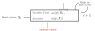
\includegraphics[width=0.7\textwidth]{module.pdf}
    \caption{Description d'une carte de Kohonen en tant que module d'une architecture modulaire. Un module prend des entrées et possède des variables d'état, ici les poids $\w$, dont l'évolution dans le temps est régie par des règles de mise à jour ou équations d'évolution.L'interface entre les modules est un ensemble de variable d'états, accessible par d'autres modules. Il peut par exemple s'agir de l'activation ou du BMU. \label{fig:module}}
\end{figure}

\subsection{\'Eléments de comparaison}

Détaillons l'approche sous laquelle nous abordons l'étude de ces architectures.
Il s'agit d'abord de différencier les architectures dédiées au traitement d'un problème particulier et les architectures génériques. Pour résoudre un problème complexe, une démarche courante est de le décomposer en sous-problèmes puis de créer des structures pour résoudre ces sous-problèmes. L'assemblage des résultats de chaque structure donne alors une solution pour résoudre le problème général. En terme d'apprentissage, il s'agit de combiner différents types de réseaux de neurones dédiés à des sous-problèmes.
Nous différencions cette vision d'architecture dédiée à une application, de la notion de modèle d'architecture.
On entend par modèle d'architecture le cadre de calcul sous-jacent au modèle, appliqué ou non, défini par ses règles de construction. Dans ce chapitre, nous nous intéressons spécifiquement aux modèles d'architectures.
Nous nous intéresserons en particulier à l'aspect modulaire de ces modèles d'architectures.
Par module, nous entendons un élément possédant des règles d'évolution temporelles, à partir d'éléments d'entrées. Nous définissons comme architecture modulaire l'assemblage de modules de même type par une interface définie. Des modules doivent pouvoir être ajoutés ou retirés à une architecture modulaire sans modifier la structure interne des autres modules de l'architecture.
Les cartes auto-organisatrices s'interprètent facilement en tant que module d'une architecture~: elles prennent des entrées $\inpx$ et ont des variables d'état $\w$ mises à jour par des règles d'évolution. La conception du modèle d'architecture consiste ensuite à définir l'interface entre les modules~: il peut s'agir de la position du BMU, des poids ou des valeurs d'activités.
Un schéma d'une carte considéré en tant que module d'une architecture est par exemple représenté en figure~\ref{fig:module}.
Nous présenterons donc dans cette section des modèles d'architectures composés uniquement de cartes auto-organisatrices, en se focalisant sur les mécanismes d'apprentissage induits par l'utilisation de plusieurs cartes combinées en tant que modules.

L'étude des architectures nous a amenée à différencier les structures selon plusieurs aspects, résumés en figure~\ref{fig:taxo}.
Nous distinguons deux structures principales d'architectures de cartes~: les architectures \emph{hiérarchiques} et les architectures \emph{non hiérarchiques}.
Une architecture est dite hiérarchique lorsqu'il n'existe pas de rétroactions, directes ou indirectes, dans les connexions entre cartes. Dans ce cas, on peut définir des niveaux de cartes. Les cartes d'un même niveau ne sont pas connectées entre elles, ont au moins une connexion arrivant du niveau précédent et/ou une connexion sortant vers le niveau suivant.
Une architecture est au contraire non hiérarchique lorsqu'il existe au moins une boucle de rétroaction. Cette boucle peut être une connexion bidirectionnelle entre deux cartes ou une boucle comprenant plus de n\oe{}uds. Ces boucles implémentent des rétroactions entre les cartes de l'architecture.
Au sein des architectures non hiérarchiques, nous différencions deux paradigmes que nous détaillerons dans la section correspondante~: les architectures centralisées et décentralisées, dont un exemple est donné en figure~\ref{fig:structure}.

Au sein de ces catégories d'architectures, nous nous intéressons à la façon dont les cartes interagissent~:
les interactions sont-elles gérées par un processus extérieur aux cartes et global à l'architecture, ou sont-elles traitées localement par les mécanismes d'organisation de chaque carte.
Nous relèverons également les éléments transmis entre les cartes~:
certaines architectures utilisent ainsi la position du BMU, son poids, ou encore un ensemble d'activités de neurones d'une carte.
Enfin, la temporalité de l'algorithme de mise à jour de l'architecture peut se présenter de différentes façons. Nous appelons mise à jour séquentielle un algorithme dans lequel l'apprentissage est complètement effectué sur un module, avant de mettre à jour les suivants. La mise à jour est synchrone lorsqu'on peut définir des itérations communes à l'architecture, pendant lesquelles tous les modules seront mis à jour. La mise à jour est asynchrone lorsqu'un module n'est mis à jour que lorsqu'un signal déclencheur lui parvient.

\begin{figure}
\centering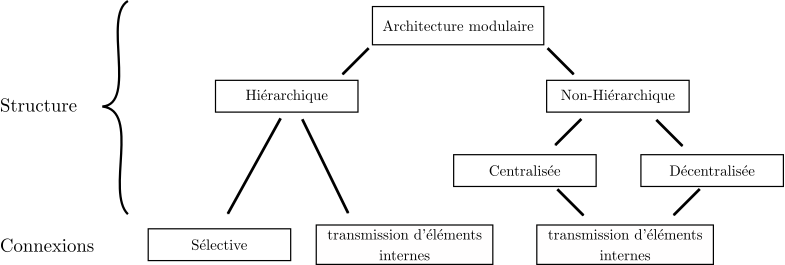
\includegraphics[width=\textwidth]{structures.pdf}
\caption{Taxonomie des architectures de cartes présentées dans ce chapitre. Nous analyserons comment leurs caractéristiques structurelles~: hiérarchiques ou non hiérarchiques, centralisées, décentralisées, façonnent leur comportement d'apprentissage. Nous analyserons également leur interface de communication. Nous n'avons pas relevé d'architecture non hiérarchique s'appuyant sur le principe de sélection, car ce principe est inhérent à une organisation hiérarchique. \label{fig:taxo}}
\end{figure}

\subsection{Architectures hiérarchiques de cartes}

Présentons d'abord les architectures hiérarchiques de cartes, qui ne présentent pas de rétroactions. Ces architectures se retrouvent également sous les termes de \emph{Deep SOM} ou SOM multicouches.
Nous avons relevé deux paradigmes de construction~: dans un premier cas, l'architecture s'appuie sur un processus extérieur aux cartes, qui sélectionne et attribue les entrées à présenter à une carte.
Dans l'autre, l'architecture est composée de cartes dont certaines apprennent les entrées externes et d'autre apprennent sur des éléments de sortie d'autres cartes.
Par facilité de représentation, les schémas des architectures seront présentés avec des cartes en une dimension. Cependant, toutes les architectures présentées utilisent des cartes en deux dimensions, parfois plus.
Le lecteur peut également se référer à \cite{henriques_spatial_2012} pour une revue des méthodes de clustering basées sur des SOMs hiérarchiques. 

\subsubsection{Architectures hiérarchiques par sélection}

\begin{figure}
    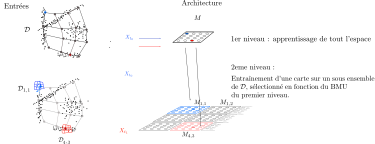
\includegraphics[width=\textwidth]{HSOM_selective.pdf}
    \caption{Exemple d'architecture hiérarchique sélective. La carte du premier niveau est entraînée sur tout l'espace d'entrée. Après apprentissage, la carte permet de filtrer les entrées pour les envoyer vers une carte du niveau suivant. Dans cet exemple, la position du BMU de la carte du niveau 1 permet de sélectionner une carte du niveau 2, comme c'est le cas en \cite{barbalho_hierarchical_2001}. 
    L'entrée permet d'entraîner une carte du deuxième niveau. Chacune des cartes du niveau 2 apprend alors sur un sous-espace d'entrée. La carte $M$ est représentée sur les données d'entrée (disposition exemple, non générée par une simulation). Le sous espace $\mathcal{D}_1$ lié au BMU à la position $1$ alimente alors une carte du deuxième niveau $M_1$.
    \label{fig:hsom_selective}}
\end{figure}

Nous appelons architecture par sélection un ensemble de cartes organisés en différents niveaux, et dont la sortie d'un niveau de cartes permet de diviser l'espace d'entrée en sous-espaces qui seront utilisés comme entrées par le niveau de cartes supérieur.
Détaillons par exemple l'architecture développée en \cite{barbalho_hierarchical_2001}, représentée en figure \ref{fig:hsom_selective}. Ce modèle est également décliné en une version dynamique dans laquelle les paramètres des cartes dépendent des données présentées, en \cite{Costa2016ANS}.
Le premier niveau de cette architecture est une carte classique, prenant des entrées $X \in \mathcal{D}$.
Une première étape consiste en un apprentissage complet de la carte du premier niveau.
Le second niveau est composé de plusieurs cartes~; chacune de ces cartes est associée à un des n\oe{}uds de la première.
Lors la deuxième phase de l'apprentissage, les données d'entrées sont réparties en plusieurs sous-ensembles, tels que chaque sous-ensemble $\mathcal{D}_i$ est l'ensemble des entrées $X_t$ ayant $i$ pour position du BMU associé à l'entrée.
Chaque carte $i$ du deuxième niveau est alors entrainée sur son espace $\mathcal{D}_i$, les cartes du premier niveau n'étant plus mises à jour.
L'architecture de cartes peut être définie à l'avance comme en \cite{barbalho_hierarchical_2001} ou de façon incrémentale en s'adaptant aux données, comme en \cite{Costa2016ANS} 
L'ensemble des prototypes des cartes, non seulement ceux du dernier niveau, forment alors une cartographie plus précise de l'espace d'entrée~: l'erreur de quantification vectorielle y est plus faible.
Ce processus est sélectif dans la mesure ou chaque carte se voit sélectionnée pour l'apprentissage d'une entrée en fonction de l'état du niveau précédent.

Ce principe se retrouve en \cite{miikkulainen_script_1992}. 
Les auteurs utilisent ici une architecture du même type mais pour traiter des données à structure hiérarchiques, ici des phrases écrites. La structure est similaire~: une carte d'un premier niveau prend une entrée qui est une phrase et permet d'extraire une représentation globale des entrées. Une fois cette carte entraînée, chaque carte du deuxième niveau apprend sur le sous-espace de phrases ayant un même BMU au premier niveau. Contrairement aux exemples précédents, les auteurs filtrent l'entrée avant de la transmettre à la carte du deuxième niveau pour en extraire les dimensions pertinentes pour le sous-ensemble en question. L'aspect hiérarchique de l'architecture permet ainsi de découvrir des motifs hiérarchiques dans la dimension des données parallèlement à leur quantification sur leur valeur.
Cette découverte de structures hiérarchiques dans les entrées se retrouve en \cite{ordonez_hierarchical_2010,dittenbach_growing_2000}.
Nous notons que le choix de répartition des sous-ensembles du deuxième niveau repose dans tous les modèles présentés ici sur la position du BMU du premier niveau, avec éventuellement des variantes comme en \cite{suganthan_pattern_2001} qui choisit de considérer plusieurs BMUs par entrée pour décomposer l'espace en sous-ensembles qui se chevauchent.

L'application privilégiée de ces architectures sélectives est d'améliorer la quantification vectorielle réalisée dans une SOM en décomposant cette quantification en un ensemble de cartes apprenant sur des sous-groupes de données détectées dans l'espace d'entrée.
Cette décomposition peut permettre la découverte de structures hiérarchiques dans les données d'entrées.
Le premier niveau seul est alors une représentation générale de l'espace d'entrée. L'augmentation du nombre de cartes et leur séparation dans les niveaux supérieurs permet une meilleure précision en termes de quantification vectorielle sur chaque sous-espace et cette division du travail réduit le coût du calcul.

Ces travaux montrent que l'agrégation de cartes de Kohonen en architecture permet d'améliorer les performances d'une SOM en tant qu'algorithme de quantification vectorielle et de diversifier les représentations extraites par la carte en y ajoutant un aspect hiérarchique.
Cependant, bien que la position du BMU soit utilisée pour la décomposition de l'espace d'entrée en sous-espaces, l'aspect de représentation topologique n'est pas spécialement exploité dans ce type d'architectures.
C'est plutôt le principe de \emph{clustering} qui permet de séparer l'espace d'entrée en sous-espaces, ainsi ce type d'architecture pourrait aussi se construire à partir d'autres algorithmes de clustering comme K-means \parencite{1094577}.

Dans notre analyse, nous ne considérons pas ces architectures comme modulaires, par l'aspect global de l'algorithme.
C'est en effet un processus extérieur aux cartes qui permet de sélectionner la carte du niveau suivant, de créer ou non des cartes à ajouter à l'architecture et de décomposer les entrées en sous-espaces. L'algorithme de mise à jour des poids de l'architecture est ainsi sous la dépendance d'un processus global.
Seul ce processus traite l'information de chacune des cartes et apporte une connexion entre cartes.

\subsubsection{Architectures hiérarchiques par transmission de représentation interne}

Certaines architectures implémentent une interface entre cartes gérée directement au niveau de l'algorithme d'organisation de la carte. La gestion de l'interface entre cartes est ainsi locale à une carte~: aucune surcouche algorithmique globale à l'architecture n'intervient dans les tâches de transmission d'information. Notons que la gestion des itérations peut rester globale à l'architecture.
Contrairement aux architectures par sélection, le deuxième niveau de cartes de ces architectures hiérarchiques ne prend plus comme entrée un élément de l'espace d'entrée de l'architecture, mais des éléments des cartes des couches précédentes, tels que la position, le poids du BMU ou un ensemble d'activation.
Ces éléments sont une représentation de l'entrée, transmise à la couche supérieure.

Des travaux proposant un modèle de SOM hiérarchique ont été développés assez tôt en \cite{luttrell_hierarchical_1989}. 
Ces travaux proposent un algorithme de quantification vectorielle hiérarchique à partir de cartes de Kohonen, et montrent expérimentalement qu'il s'agit d'une méthode moins coûteuse qu'une SOM classique pour quantifier des données de grande dimension. Notons que ces travaux ne sont pas applicables seulement aux SOMs mais à tout algorithme de quantification vectorielle. Les auteurs utilisent ici le poids du BMU comme interface entre les SOMs.

Parmi ces premiers travaux, le modèle HSOM \parencite{lampinen_clustering_1992} construit une architecture composée de deux cartes~: une première carte $M\m{1}$ se déplie sur des entrées $\inpx\m{1}$, et une deuxième carte $M\m{2}$ reçoit ensuite comme entrée $\inpx\m{2}$ la position du BMU $\bmu\m{1}$ de la première carte~; cette architecture est illustrée en figure~\ref{fig:hsom}.
Le BMU de la première carte est alors défini par~:
$$ \Pi\m{1} = \argmin_p(||\w\m{1}(p) - X\m{1} || ^2)$$
Le BMU de la deuxième couche est ensuite calculé comme~:
$$ \Pi\m{2}= \argmin(||\w\m{2}(p) - \Pi\m{1} || ^2)$$
La deuxième carte réalise ainsi de la quantification vectorielle sur les positions du BMU de la première carte. Les auteurs utilisent HSOM dans le cadre du \emph{clustering} et la classification de données~: les SOMs doivent automatiquement extraire des groupes de données (\emph{clusters}) par similarité, sachant que les données sont effectivement regroupées en classes distinctes. Ces clusters sont définis après apprentissage par les cellules de Voronoi dont les poids de la carte $\w(p)$ en sont les centres.
Comme les cartes s'organisent de façon à conserver les distances dans l'espace d'entrée au sein de la carte, deux éléments faisant partie d'un même cluster auront des BMUs proches dans la première carte~; par conséquent, leurs BMUs dans la seconde carte le seront également. 
Ils notent que la SOM du premier niveau de l'architecture, qui est une SOM classique, générera de nombreux petits clusters, dont plusieurs d'entre eux seront nécessaires pour couvrir une classe entière. Au contraire, la deuxième couche de SOMs génère des clusters plus larges, et moins de ces clusters seront alors nécessaires pour couvrir une classe de données.
Le fait d'utiliser une architecture de SOMs permet dans ce cas d'extraire une représentation différente de celle extraite par une SOM classique.

\begin{figure}[t]
    \centering
    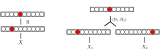
\includegraphics[width=\textwidth]{HSOM.pdf}
    \caption{Deux exemples d'architectures basées sur HSOM. A gauche, le modèle HSOM original proposé en \cite{lampinen_clustering_1992}. L'apprentissage des positions du BMU de la première couche par la seconde permet de mieux détecter les ensembles de données présents dans la distribution des $X$ (\emph{clustering}).
    La deuxième couche est vue comme un niveau plus abstrait que la première. 
    \`A droite, une version de HSOM comportant plus de cartes proposée en \cite{hagenauer_hierarchical_2013} permettant de faire du clustering sur des entrées provenant de deux espaces $X_1\m{1}$ et $X_2\m{1}$. Ces deux espaces sont ici des caractéristiques spatiales et temporelles d'un environnement d'entrée.
    \label{fig:hsom}}
\end{figure}


D'autres travaux par la suite implémentent des modèles similaires transmettant la position du BMU entre cartes, sur des architectures comportant plus de cartes que HSOM, tel que \cite{hagenauer_hierarchical_2013, Paplinski2005MultimodalFS}.
Dans leurs travaux, les auteurs implémentent une architecture en arbre. La carte du niveau $i$, $M\m{i}$ reçoit alors un vecteur de position de BMUs de $k+1$ cartes $M_0\m{i-1}, \cdots, M_k\m{i-1}$  du niveau inférieur en tant qu'entrée~:
$$ \inpx\m{i} = [\Pi_0\m{i-1}, \cdots, \Pi_k\m{i-1}]$$
L'architecture est dans ce cas utilisée pour l'agrégation de données dépendantes les unes des autres.
La carte du niveau supérieur apparaît comme une représentation abstraite des données et de leurs dépendances.


Un point clé dans la construction de ces architectures repose sur l'information transmise entre couches. 
Cette information doit permettre de véhiculer un maximum d'information entre cartes, tout en étant interprétable par les autres cartes.
Les architectures HSOM et ses dérivées utilisent ainsi la position du BMU en tant que représentation.
Par le choix de la position du BMU comme vecteur de transmission d'information, HSOM exploite effectivement sur la préservation de la topologie de l'espace d'entrée qu'offrent les cartes de Kohonen.
Cette information est par ailleurs relative à une carte et non un type d'entrée. Enfin, il s'agit d'une position 1D ou 2D, donc une information peu coûteuse à utiliser.
Nous avons également relevé le poids du BMU $\w(\bmu)$ comme une méthode de transmission d'information au sein d'autres modèles de SOMs hiérarchiques, comme \cite{wang_comparisonal_2007, gunes_kayacik_hierarchical_2007, dozono_convolutional_2016}.
Par exemple, \cite{dozono_convolutional_2016} décomposent une image d'entrée en imagettes qui sont utilisées en tant qu'entrées d'une première couche de cartes. 
Après apprentissage de cette couche, l'image est reconstruite grâce aux poids des BMU, puis décomposée en imagettes de tailles différentes pour être soumise à la deuxième couche de cartes.
Enfin, les travaux de~\cite{mici_self-organizing_2018} s'appuient sur des cartes hiérarchiques pour effectuer de la fusion de données spatio-temporelles.
Les auteurs et autrices de ces travaux utilisent comme sortie de la carte temporelle la série de poids des BMU successifs, relatifs à la séquence d'entrée, et comme sortie de la carte spatiale le poids du BMU relatif à l'entrée. L'entrée de la deuxième couche de cartes est alors un mélange entre les deux modalités. L'application de cette architecture mérite d'être soulignée, dans la mesure où elle permet d'associer information spatiale et temporelle.


Le terme de \emph{Deep SOM} est régulièrement rencontré lorsqu'on s'intéresse aux travaux récents portant sur les architectures de cartes auto-organisatrices.
Aussi \cite{liu_deep_2015, dozono_convolutional_2016, hankins_somnet_2018, mici_self-organizing_2018, wickramasinghe_deep_2019, aly_deep_2020,sakkari_convolutional_2020,,nawaratne_hierarchical_2020-1} et de nombreux autres travaux sont présentés comme tels.
Les travaux se décrivant par ces termes implémentent des structures hiérarchiques puisant leur inspiration des réseaux de neurones profonds (\emph{Deep Learning}), ayant notamment connu leur essor avec les réseaux convolutifs permettant l'apprentissage supervisé d'images \parencite{lecun_deep_2015}. 
Cependant, leur analogie avec les modèles de Deep Learning, qui s'appuient sur le principe de rétropropagation du gradient, s'arrête à la présence de couches de poids et leur application au traitement d'image. Dans leur structure, les modèles de Deep SOM restent bien proches des modèles de SOM et SOM hiérarchiques.
Par analogie avec ces réseaux convolutifs, les réseaux présentés comme Deep SOM s'intéressent à l'apprentissage d'images.

Nous pouvons prendre comme exemple le modèle D-SOM introduit en \cite{liu_deep_2015,wickramasinghe_deep_2019}, illustré en figure~\ref{fig:dsom}.
Le but d'une telle architecture est de classifier des images $X$ fournies en entrée de l'architecture.
Une fenêtre est déplacée sur l'image d'entrée, créant un ensemble de $N\times N$ imagettes de position fixée. La première couche du réseau comporte $N \times N$ cartes, donc chacune prend en entrée l'imagette de même position $i,j$.
La sortie de la couche donne $N  \times N$ positions de BMU $\bmu_{i,j}$.
Ces positions représentées comme des valeurs en une dimension sont assemblées en une image intermédiaire, chaque pixel prenant la valeur du BMU de la carte correspondante.
    $$X_{int} = \begin{pmatrix}
    \bmu_{0,0}  &  \cdots & \bmu_{0,N} \\
    \cdots & \cdots & \cdots \\
    \bmu_{N,0} & \cdots & \bmu_{N,N}
    \end{pmatrix} $$

Une deuxième couche de cartes de même structure que la première carte est alors appliquée à cette image intermédiaire. La dernière couche du réseau est composée d'une SOM simple effectuant la quantification vectorielle sur l'image de sortie de la couche précédente, vue comme une représentation abstraite de l'entrée.
L'interface entre les couches de cartes est créée à partir des BMUs des SOMs~: ce modèle de transmission rejoint ainsi ceux présentés dans HSOM. La différence apparaît au niveau du prétraitement de l'entrée image, décomposée en imagettes.

Ce type d'architecture utilise bien l'aspect topologique de la carte de Kohonen dans ses calculs, les interfaces entre couches de cartes s'appuyant sur les positions du BMU. L'utilisation des positions au lieu de poids permettent de réduire la dimension des images traitées par les couches successives. L'image de sortie de la dernière couche est alors de taille réduite. Lorsque la dernière SOM classifie les images générées par la dernière couche, elle classifie une représentation plus abstraite de l'image d'entrée. L'étude montre que la classification de cette dernière image permet de bien retrouver les classes présentes dans les données d'entrées. Les auteurs notent que l'architecture D-SOM possède une erreur de classification sur MNIST plus faible qu'une SOM simple, ce qui montre que l'abstraction générée par les couches successive renforce la séparation entre classes.
Par l'assemblage des positions du BMU en tant que représentation intermédiaire de l'entrée, l'architecture D-SOM est très similaire à HSOM.

\begin{figure}[t]
    \includegraphics[width=\textwidth]{DSOM.pdf}
    \caption{Architecture DSOM de SOM \og convolutive \fg{} \parencite{liu_deep_2015}. Les auteurs utilisent les positions des BMUs $\Pi_{p,q}$ d'une couche de carte, disposés dans un tableau 2D, comme valeurs d'entrée pour les couches suivantes. Ces couches sont entraînées les unes après les autres. \label{fig:dsom}}
\end{figure}

Toutes les architectures présentées ici, qu'il s'agisse des SOMs hiérarchiques ou Deep SOM, comme pour les architectures sélectives, sont ascendantes dans leur mise à jour~: chacune des couches de cartes est entraînée l'une après l'autre. 
Si les tâches de classifications réalisées par ces travaux auraient pu être réalisées avec une SOM classique, l'utilisation d'une architecture plutôt qu'une SOM donne de meilleures performances en termes d'erreur de classification.

\subsubsection{Discussion}

Nous avons distingué deux catégories d'architectures hiérarchiques en nous appuyant sur le mode de connexion entre cartes dans l'algorithme de mise à jour. 
Le premier mode de connexion repose sur la sélection d'une carte du niveau supérieur en s'appuyant sur la réponse des cartes d'un même niveau à une entrée, afin de transmettre cette entrée à la carte supérieure. Ce mode de transmission permet de créer un ensemble de cartes s'organisant sur un même espace d'entrée, laissant plus de possibilités au dépliement des cartes qu'une SOM classique. Ces types d'architectures permettent notamment d'améliorer la qualité de la quantification vectorielle générée par une SOM classique et d'ajouter des n\oe{}uds de façon peu coûteuse. Le mode de transmission par sélection s'appuie sur une surcouche algorithmique aux cartes, qui décompose successivement l'espace d'entrée en sous-espaces et distribue aux cartes leurs entrées. Ce type d'architecture n'est pas modulaire dans la mesure ou la connexion entre carte est gérée par un processus global.

Le second mode de connexion repose sur la modification du principe de calcul d'activité et de mise à jour d'une carte pour prendre en compte les éléments de réponse d'une autre carte, par exemple en ajoutant cet élément de réponse en tant qu'entrée secondaire d'une carte.
Ce mode de connexion est intégré au processus d'auto-organisation, il ne s'agit pas d'une couche algorithmique supplémentaire comme pour les architectures par sélection, ce qui localise le traitement des connexions à l'échelle d'une carte. 
Cette méthode de construction d'architecture s'appuie sur la transmission d'une représentation de l'entrée interne entre cartes.
Ce type de connexions nous intéresse d'un point de vue modulaire~: il autorise l'ajout de modules à une architecture sans avoir à modifier toute la structure de l'architecture, ce qui est un des éléments de définition d'un système modulaire.
Nous verrons plus loin que les architectures non hiérarchiques s'appuient toutes sur ce mode de transmission.
Nous avons relevé au sein des architectures hiérarchiques deux représentations internes majoritairement utilisées comme information transmise entre cartes~: la position du BMU ou le poids du BMU. La position du BMU est une représentation exploitant totalement l'aspect topologique d'une carte auto-organisatrice, de dimension faible et homogène à toutes les cartes. Il permet aussi d'extraire une représentation abstraite de l'entrée, ce qui est le but recherché d'une architecture, par exemple dans le cas de la classification de données multimodales.
En revanche, lorsque le poids du BMU est échangé, les calculs sont plus coûteux. On perd l'aspect générique et homogène de la transmission des positions des BMU, ce qui oblige à particulariser les calculs. Cet échange de poids n'exploite pas l'aspect topologique d'une carte de Kohonen, mais seulement sa capacité de quantification vectorielle.
Nous reviendrons sur ces modes de représentations en analysant les architectures non hiérarchiques.

Qu'elles soient sélectives ou par transmission de représentation, toutes les architectures relevées ici ont une séquence de mise à jour séquentielle~: les cartes du premier niveau sont dépliées lors d'une première phase d'apprentissage. Une fois ces cartes dépliées, la deuxième couche est apprise à partir de la première lors d'une deuxième phase, lors de laquelle le premier niveau n'est plus mis à jour.
Le champ d'application des architectures hiérarchiques est le même qu'une SOM classique~: quantification vectorielle et classification.
Dans les deux cas, il s'agit d'améliorer les performances sur une tâche de quantification vectorielle ou de classification pouvant être réalisée par une SOM. 
Par exemple, les SOMs par sélection permettent d'améliorer la quantification vectorielle sur l'espace d'entrée ou de prendre en compte l'aspect hiérarchique des entrées. Les SOMs par transmission de représentation permettent de mieux isoler les clusters de données qu'une SOM classique ou d'effectuer une classification sur des données multimodales.
Nous pouvons donc considérer ces architectures comme des améliorations de cartes auto-organisatrices sur des applications spécifiques.
Elles ont les mêmes type de réponses qu'une SOM simple.
L'aspect uniquement ascendant en est la cause~: les cartes de l'architecture agissent comme des filtres intermédiaires de l'information donnée en entrée, mais seule la couche finale est considérée en sortie de l'architecture : cette couche finale reste une carte auto-organisatrice classique, apprenant simplement sur des entrées filtrées.
Dans une volonté d'étudier une architecture proposant des comportements de calcul différents de ceux réalisés dans une SOM classique, notre attention se portera sur les architectures comportant des boucles de rétroaction~: les architectures non hiérarchiques.
Ces architectures permettent de diversifier les comportements d'apprentissage qu'il est possible d'obtenir avec des SOMs en apportant un aspect dynamique au système par les rétroactions. 
Notons qu'une architecture hiérarchique est un cas particulier d'architecture non hiérarchique~: les modèles que nous allons étudier en partie suivante pourraient donc aussi bien être utilisés dans un cadre hiérarchique.


\subsection{Architectures non hiérarchiques de cartes auto-organisatrices}

\begin{figure}
    \centering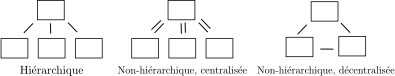
\includegraphics[width=0.8\textwidth]{structures_002.pdf}
    \caption{Exemples de connexions dans des architectures hiérarchiques et non hiérarchiques centralisées et décentralisées. Un rectangle correspond à un module, ici une carte auto-organisatrice. Une flèche représente l'existence d'une interface entre deux modules~: le module destination prend comme entrée contextuelle la sortie de la source et utilise donc de l'information de la source dans ses règles d'évolution. \label{fig:structure}}
    \end{figure}


Les architectures non hiérarchiques de SOMs sont des architectures comportant plusieurs cartes communiquant entre elles et dont le graphe de connexion comporte des boucles de rétroaction~: une carte A reçoit de l'information d'une carte B, qui elle-même reçoit, directement ou indirectement, de l'information de la carte A.

Notons d'abord que les travaux cherchant à assembler des réseaux de neurones en architecture non hiérarchiques se revendiquent plutôt du domaine des neurosciences computationnelles ou de la robotique, tandis que les architectures hiérarchiques décrites précédemment se positionnaient dans un domaine d'apprentissage automatique, dans un objectif d'amélioration de la classification et quantification vectorielle d'une SOM.
Les motivations se situent d'une part au niveau de l'inspiration biologique des modèles. 
Nous avons vu que le cortex présente des aires dont les activités sont corrélées, suggérant une relation entre les activations des différentes aires. Ces relations sont observées comme bidirectionnelles et intervenant à différents niveaux du traitement de l'information sensorielle.
Les travaux de modélisation du cerveau cherchent donc à implémenter des architectures de réseaux de neurones non hiérarchiques. 
Nous ne détaillerons pas ici les travaux portant sur des modélisations fines du cerveau à base de modèles biologiques de neurones, nous intéressant seulement à ceux présentant des cartes auto-organisatrices.
Nous avons par contre vu qu'une carte de Kohonen, sans être une modélisation fine d'une aire cérébrale, est une adaptation informatique d'un concept d'auto-organisation présent dans les aires sensorielles des réseaux de neurones biologiques. Plusieurs travaux de neurosciences computationnelles ont ainsi utilisé des cartes de Kohonen comme un modèle simplifié d'aire cérébrale pour les assembler en architecture.


L'aspect bio-inspiré se retrouve également dans les motivations des modèles robotiques. Ces modèles se placent dans le paradigme d'embodiment (\emph{Embodied Cognition}), c'est-à-dire le développement d'un système intelligent qui peut interagir avec son environnement. Parmi les éléments de recherche principaux de ce domaine robotique figurent la fusion de données multimodales, le traitement de séquences et l'apprentissage développemental, inspiré du comportement des humains et animaux. \parencite{Smith2005TheDO}.
Le recensement des architectures de cartes non hiérarchiques relève ainsi de plusieurs domaines, dans la mesure où ces modèles sont développés dans le contexte des neurosciences computationnelles ou de la robotique cognitive et cherchent à modéliser les aires cérébrales. 
Nous chercherons à faire une relecture de ces modèles d'un point de vue de la méthode de transmission d'information entre les cartes de ces structures, comme nous l'avons réalisé sur les architectures hiérarchiques.
Toutes ces architectures non hiérarchiques ont en commun leur champ d'application~: contrairement aux architectures hiérarchiques ascendantes qui cherchent à améliorer les performances de classification ou de \emph{clustering} d'une SOM classique, les SOM non hiérarchiques que nous avons relevées dans la littérature sont plutôt appliquées à des tâches de \emph{mémoire associative} sur des données \emph{multimodales}.
Ces cartes sont des systèmes dynamiques par leurs rétroactions et ont la capacité de générer une valeur de sortie de façon autonome. Elles sont alors utilisées pour prédire une modalité à partir d'une autre, ce qui correspond à une tâche de mémoire associative.


Nous avons pu distinguer deux structures principales d'architectures non hiérarchiques dans les travaux réalisés jusqu'à présent, illustrées en figure~\ref{fig:structure}.
Certaines architectures comportent des cartes sensorielles qui sont reliées via des cartes associatives ne prenant pas d'entrées sensorielles, mais seulement des éléments de connexion contextuels. 
Ces architectures sont \emph{centralisées}, étant donné que les cartes associatives centralisent l'information  montant des cartes sensorielles et la redistribuent. Ces architectures centralisées sont souvent désignées par leurs auteurs comme hiérarchiques~: en effet, les cartes associatives forment un niveau d'apprentissage différent des cartes sensorielles, apportant une hiérarchie dans l'apprentissage. 
Néanmoins, nous les classons ici dans la catégorie non hiérarchique. 
En effet, bien que des niveaux de cartes peuvent être isolés dans ces architectures, les connexions entre les cartes de deux niveaux sont bidirectionnelles, la carte associative étant à l'origine de l'activation de cartes sensorielles, et réciproquement.
Nous les différencions ainsi des cartes hiérarchiques uniquement ascendantes que nous avons listées au paragraphe précédent.
Un second type d'architectures non hiérarchiques sont les architectures présentant des connexions directes entre cartes sensorielles. Ces architectures sont \emph{décentralisées}, pour lesquelles il n'existe pas de module par lequel toute l'information transite.

\subsubsection{La mémoire associative et l'apprentissage développemental comme applications des architectures non hiérarchiques}

Les architectures non hiérarchiques proposées dans la littérature ont en commun leur application à la mémoire associative de données multimodales.
La fusion de données multimodales est un enjeu actuel des algorithmes d'apprentissage en robotique développementale.
Il s'agit d'intégrer les données issues de multiples capteurs au sein d'un même algorithme d'apprentissage.
Il est en effet rare que l'information issue d'un seul capteur apporte toute l'information nécessaire à l'apprentissage et la prise de décision dans un environnement réel \parencite{lahat2015}. 
%Notre comportement est multisensoriel, influencé par toutes les sources d'informations dont nous disposons.

Dans la mesure où la recherche en robotique cherche à complexifier les comportements possibles pour les agents et à s'inspirer de la biologie, la prise en compte de données de différentes sources est nécessaire. Ces données proviennent d'espace de différentes dimensions comme des images, des capteurs audio, des capteurs tactiles, du texte, des actions. Leur temporalité peut varier~: on veut pouvoir associer des données séquentielles, c'est-à-dire extraire de l'information d'une succession d'entrées, à des données instantanées dans lesquelles seule la valeur de l'entrée compte. La fréquence d'arrivée des données séquentielles varie également.
L'enjeu de la fusion de données multimodales est alors de concilier tous ces aspects lors de l'apprentissage.

La mémoire associative se définit dans le cadre de la fusion de données multimodale par l'action de prise de décision sur une modalité relativement aux autres.
Les autres modalités peuvent venir améliorer la prise de décision par rapport à la modalité seule. C'est par exemple le cas dans l'effet McGurk \parencite{McGurk1976HearingLA}, lorsque la vision d'une bouche prononçant "ga" associée au son "ba" amène un sujet à indiquer avoir entendu "da" (voir section \ref{sec:bioinspi}. Il est également montré que le fait de lire sur les lèvres en écoutant une personne améliore la compréhension du discours, par exemple dans un environnement bruyant. Il s'agit ici de mémoire associative entre modalités visuelles et auditives.
Cette mémoire associative peut aussi s'utiliser pour prédire une modalité par rapport aux autres~: les modalités visuelles et auditives vont générer une prise de décision au niveau de la modalité moteur d'un robot et ainsi générer une action par association.

Les architectures de cartes non hiérarchiques que nous avons relevées se positionnent dans un cadre de mémoire associative, que ce soit par une motivation bio-inspirée ou par leur but d'implémentation en robotique.
Leur architecture modulaire apparaît comme un moyen de réaliser de la fusion de données à l'échelle de l'algorithme, par opposition à la fusion de données à l'échelle des entrées. 
Une modalité est alors traitée par un ensemble de cartes de l'architecture, et les autres cartes de l'architecture n'ont accès qu'à une information filtrée de cette entrée. 


Notons que les cartes hiérarchiques apparaissaient déjà comme un moyen de traiter des données multimodales, par exemple en \cite{mici_self-organizing_2018} et \cite{nawaratne_hierarchical_2020-1}. 
Une carte traite des données spatiales d'un côté, une autre des données temporelles~; l'architecture associe la sortie de ces cartes dans la couche finale pour classifier les motifs spatio-temporels. Les cartes du premier niveau étaient alors consacrées à la représentation d'une modalité, tandis que la dernière carte est une carte associative apprenant des motifs spatio-temporels liant les deux cartes modales.
Les cartes non hiérarchiques vont plus loin dans l'application de la mémoire associative, car la présence de rétroactions permet de générer une activité au sein d'une carte modale par ses connexions aux autres cartes, même lorsque l'entrée est manquante.
Une carte auto-organisatrice acquiert ainsi une capacité de prise de décision, par son activation alors que la carte hiérarchique permet seulement d'extraire une représentation.
Cette activation étant lié à des poids représentant la modalité, il est alors possible de prédire une valeur pour la modalité manquante. 
Cette prédiction de modalité est utilisée dans les différents travaux présentés dans cette section comme l'application principale de ce type d'architecture et les expériences de validation sont menées autour de la capacité d'une carte modale à prédire de façon précise la modalité à partir des connexions associatives.
Notons enfin que la notion de mémoire associative s'étend à l'apprentissage de séquences~: il s'agit alors d'extraire une représentation d'une séquence temporelle complète ou de pouvoir compléter automatiquement une séquence.

Le concept d'apprentissage  développemental est un autre enjeu de la robotique et s'intéresse à des systèmes étant mis à jour en ligne, dès qu'ils reçoivent une entrée, et dont l'apprentissage n'a pas de limite temporelle fixée. On doit donc avoir un système qui trouve de lui-même une stabilité dans l'apprentissage et qui est capable de s'adapter à de nouvelles entrées.
Dans les applications de robotique, les entrées présentées à une structure d'apprentissage sont des entrées ayant une relation temporelle. Deux images reçues successivement par un capteur visuel seront proches dans l'espace des images. Pour une SOM classique par exemple, cela pose problème~: le réseau s'organiserait d'abord sur le sous-espace composé des premières images de la séquence, puis évoluerait en même temps que les entrées en oubliant la séquence vue précédemment.
Les architectures développementales cherchent donc une solution à ces problèmes pour créer une structure autonome, évoluant dans le temps et permettant de réaliser la tâche pour laquelle elle est conçue tout en continuant à être mise à jour, sans oublier catastrophiquement les données apprises au début de l'apprentissage.
Ces enjeux applicatifs, communs aux architectures présentées dans cette partie, nous motivent également à étudier les cartes non hiérarchiques.

\subsubsection{Architecture comportant une carte associative~: architecture centralisée}

L'idée d'assembler des cartes prenant en entrée une modalité sensorielle par une carte associative a été explorée en \cite{dominey13} et \cite{escobar-juarez_self-organized_2016}.
Dans ces deux travaux de neurosciences computationnelles, les auteurs construisent une architecture se voulant une modélisation de la théorie de la zone de convergence-divergence \parencite{Edelman1982GroupSA} avec des cartes auto-organisatrices, en transmettant les positions des BMU entre les cartes multimodales. 

Le modèle MMCM de \cite{dominey13} propose une architecture composée de plusieurs cartes modales chacune associée à une modalité sensorielle et d'une carte associative prenant en entrée les positions des BMU des cartes modales. Cette architecture est représentée en figure~\ref{fig:mmcm}. 
Nous définissons cette architecture comme non hiérarchique, car il existe des rétroactions entre les cartes modales $M\m{1},M\m{2}$ et la carte associative $M\m{m}$.
Dans l'exemple d'une architecture à deux cartes modales, l'une reçoit les mouvements de tête d'un robot et une autre les mouvements du bras.
Chaque carte du premier niveau possède une couche de poids $\w_e$ liées aux entrées sensorielle ainsi qu'une couche de poids $ \w_c$ dédiée aux connexions descendantes, prenant en entrée les positions du BMU de la carte associative.
La carte associative prend deux couches de poids, chaque couche correspondant à la position du BMU d'une carte sensorielle.

\begin{figure}[t]
    \centering
    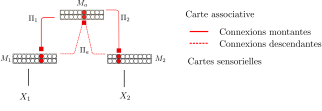
\includegraphics[width=\textwidth]{MCMM.pdf}
    \caption{L'architecture MMCM \parencite{dominey13} est une architecture centralisée.
    Les cartes du premier niveau sont les cartes modales $M\m{1}, M\m{2}$ qui reçoivent l'une les mouvements de tête d'un robot, une autre les mouvements de son bras
    Une carte associative $M\m{m}$ reçoit les positions des BMUs $\bmu\m{1},\bmu\m{2}$ de chaque carte du premier niveau en tant qu'entrées. 
    Les cartes modales ont ensuite une couche de poids encodant les positions des BMUs de la carte associatives et permettant leur activation depuis la carte associative.
    \label{fig:mmcm}}
\end{figure}

La mise à jour est réalisée en trois étapes~: 
D'abord, les couches de poids externes des cartes modales sont mises à jour indépendamment sur les entrées. La recherche du BMU est réalisée en prenant en compte une activation $a(p, \w, X\m{i})$ dans la carte.
Ensuite, les poids $\w_e$ sont ensuite gelés, et les poids de la carte associative sont mis à jour de façon à apprendre à associer les positions des BMUs $(\bmu\m{1},\bmu\m{2})$ correspondant aux cartes modales, rappelant les modèles hiérarchiques HSOM. La carte prend en entrée $\inpx\m{m} = [\bmu\m{1}, \bmu\m{2}]$

Dans un troisième temps, les poids de la carte associative sont figées et les couches de chaque carte modales $\w_c$ dédiées aux connexions sont mises à jour, l'entrée étant le BMU de la carte associative $\bmu\m{m}$.
\begin{equation*}
    \begin{cases}
        \bmu_c\m{1} = \argmax_p a(p, \bmu\m{m}, \w_c\m{1})\\
        \bmu_c\m{2} = \argmax_p a(p, \bmu\m{m}, \w_c\m{2})
    \end{cases}
    \end{equation*}

Une carte modale a donc à la fois un BMU relatif aux activités externes et un BMU $\bmu_c$ relatif aux activités contextuelles pendant l'apprentissage, les deux couches de poids étant décorrélées.
La rétroaction entre les cartes est en fait découplée lors de la phase d'apprentissage, car la carte associative dépend seulement de la couche externe des cartes sensorielles et transmet des informations seulement à la couche contextuelle des cartes sensorielles.
Après ces trois phases d'apprentissage, les entrées modales ne sont pas présentées aux cartes modales. L'activation manuelle d'un neurone de position $p\m{m}$ de la carte associative entraîne une activité et un BMU dans les deux cartes modales grâce au calcul de l'activation sur la couche de poids contextuelle~: 
$$ \bmu_c\m{1} = \argmax\limits p a(p\m{m},\w_c\m{1}(p))$$
La valeur $\w_e\m{1}(\bmu_c\m{1})$ est alors une prédiction de la modalité 1.
Les auteurs montrent que cette méthode d'activation produit des mouvements coordonnés entre modalités.
De la même façon, l'activation d'un neurone d'une carte sensorielle entraîne également une activation coordonnée dans les autres cartes sensorielles en passant par la carte associative.
Notons que les cartes utilisées dans ces travaux sont des cartes 3D.


L'architecture SOIMA \parencite{escobar-juarez_self-organized_2016} associe également plusieurs cartes modales avec une carte associative, présentée en figure \ref{fig:SOIMA}.
La transmission d'information des cartes modales vers la carte associative est réalisée par la transmission de la position du BMU~: la carte associative prend en entrée $(\Pi\m{1},\Pi\m{2})$, le couple de BMU des cartes modales. 
Afin de gérer les rétroactions, les auteurs ajoutent en tant que connexions descendantes des connexions pondérées neurone à neurone mises à jour par une règle de transmission Hebbienne~: le poids de la connexion est renforcé si les deux neurones reliés s'activent lors de la même itération.
Les connexions montantes et descendantes sont ici encodées de manière différente~; cela permet aux auteurs d'effectuer la mise à jour des cartes et de leurs connexions en une seule étape. 
Dans ces travaux, les auteurs associent deux modalités sensorielles et motrices par une carte associative en trois dimensions.
L'utilisation de connexions hebbiennes pondérées entre neurones est équivalente à transmettre l'entièreté de l'activation de la carte associative à une carte sensorielle.
Prenons l'exemple de cartes 1D. Chaque neurone $j$ de la carte modale reçoit un signal $a_{i}$ de chacun des neurones $i$ de la carte associative par une connexion de poids $\w_{ij}$. Tous les neurones de la carte modale reçoivent donc le même ensemble d'entrées $ \{a_{i},\: i = 0 .. N\}$.
Les poids des neurones $\w_i$ sont ainsi équivalent à l'ajout d'une couche de poids supplémentaire à la carte modale telle que~: $\forall j, \: \w_j \in [0,N]$ apprend un champ d'activation de la carte associative.

L'information transmise entre cartes dans l'architecture SOIMA repose sur la position du BMU pour les connexions montant des cartes sensorielles à la carte associative, et sur des champs d'activité neuronales pour les connexions descendantes.
La gestion des rétroactions est réalisée de la même façon que pour MMCM~: les couches de poids des cartes modales étant décorrélées lors de l'apprentissage, les rétroactions n'ont pas d'influence sur la mise à jour. Elles sont utilisées seulement en phase d'application.

\begin{figure}[t]
    \centering
    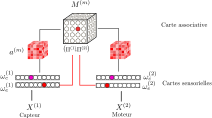
\includegraphics[width=0.8\textwidth]{SOIMA.pdf}
    \caption{Le modèle SOIMA \parencite{escobar-juarez_self-organized_2016} propose une architecture centralisée dans laquelle des cartes modales $M\m{1}$ et $M\m{2}$ sont connectées par une carte associative $M\m{a}$. Cette carte associative prend comme entrée les BMUs des cartes modales. 
    Les connexions descendantes sont gérées par la transmission du champ d'activation de $M\m{m}$ vers les cartes modales. Les poids de ces connexions sont stockés dans une deuxième couche de poids.
    \label{fig:SOIMA}}
\end{figure}

Les modèles mentionnés ci-dessus entrent dans la catégorie non hiérarchique pour leur possibilité d'activation d'une carte par l'autre. 
La position du BMU apparaît dans les modèles SOIMA et MMCM comme le vecteur de transmission d'information  entre cartes.
Le modèle SOIMA privilégie la connexion neurone à neurone entre la carte associative et la carte modale.
La présence de cartes associatives au sein d'une architecture crée une centralisation de l'information multimodale sur une carte, ce qui nous amène à parler d'apprentissage centralisé. 
Chaque carte sensorielle ne reçoit aucune information directe d'autres cartes de l'architecture, sauf de la carte associative.
Les cartes modales et associatives jouent ainsi un rôle différent dans les calculs.

La présence de rétroactions soulève une problématique de conception supplémentaire dans les cartes non hiérarchiques~: l'activité de la carte A influence l'activité de la carte B, mais l'activité de la carte B influence également celle de la carte A, etc. 
Pour résoudre ce problème, l'architecture MCMM et l'architecture SOIMA décorrèlent les couches de poids prenant en compte l'entrée modale et celles relatives à l'entrée descendant de la carte associative lors de l'apprentissage.
L'entrée de la carte associative est seulement le BMU de la couche de poids externes des cartes modales. La couche de poids contextuelle des cartes modales a son propre BMU pour la mise à jour. 
Par ailleurs, les auteurs de ces travaux décomposent l'apprentissage en plusieurs étapes~: les cartes modales sont apprises, puis la carte associative, puis les connexions descendantes. La mise à jour est donc séquentielle.

Ces modèles sont des architectures modulaires. Toutes les cartes d'une architecture ont une structure similaire. Cependant, elles prennent des rôles conceptuellement différents par leur position dans l'architecture~: certaines cartes sont associatives et d'autres cartes sont modales.

\subsubsection{Architectures non hiérarchiques décentralisées}

Une architecture non hiérarchique décentralisée est une architecture présentant des rétroactions entre cartes et dont les cartes modales présentent des connexions directes entre elles.
Les modèles d'architectures décentralisées sont les plus génériques dans la mesure où ils n'imposent pas de structure spécifique pour l'architecture.
La structure des connexions entre cartes devient alors un paramètre sur lequel on peut complètement agir, contrairement aux architectures centralisées. 
Ces modèles apparaissent comme des architectures modulaires idéales, car aucun a priori n'est associé aux modules, même une fois connectés. Leur spécialisation intervient uniquement grâce à leurs règles d'évolution internes.

Les auteurs de \cite{khacef_brain-inspired_2020} utilisent par exemple deux cartes de Kohonen associées par des connexions tous à tous entre neurones. Une carte prend en entrées des images MNIST, et l'autre le son du chiffre prononcé. L'apprentissage des deux cartes modales est réalisé dans un premier temps, puis les connexions entre neurones sont mises à jour dans une seconde étape à partir des mêmes paires d'entrées image-son. Les neurones de chaque carte s'activant sur une même paire d'entrées voient le poids de leur connexion se renforcer, et inversement. Les auteurs utilisent ici la transmission d'un champ d'activité neuronale comme vecteur de communication entre cartes (nous avons vu en effet que la connexion neurone à neurone revenait à transmettre un champ d'activation).
Après apprentissage, la présentation d'une image à la carte associée permet de générer une activité cohérente dans la carte associée au son. Le modèle a donc ainsi appris les relations existant entre les deux modalités et est capable de générer une prédiction dans une carte à partir de l'autre.
Un modèle similaire d'architecture non hiérarchique de deux cartes par transmission d'activité neuronale est également proposé en \cite{jayaratne_bio-inspired_2018}, les auteurs utilisant cette fois des SOM incrémentales au lieu de SOM à taille fixe.

\begin{figure}
    \centering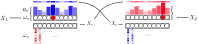
\includegraphics[width=\textwidth]{ASOM.pdf}
    \caption{Le modèle A-SOM \parencite{johnsson_associative_2009} associe les activités de différentes cartes. Chaque carte prend une entrée modale $X_1$ ou $X_2$. Chacune des cartes possède deux couches de poids, une couche $\w_e$ associée aux entrées modales et une couche $\w_c$ associées aux entrées $\inpc$ venant de l'autre carte. Lors de l'apprentissage, le calcul des activités sur chaque couche de poids est déconnecté, ce qui permet de gérer les rétroactions. 
    Après apprentissage, une des entrées est supprimée. L'activation de la carte correspondante est alors permise par les connexions contextuelles, amenant la carte à prédire une entrée. Les cartes sont représentées en version 1D pour plus de clarté, mais le modèle utilise des cartes 2D.
    \label{fig:asom}}
\end{figure}

Une autre version d'architecture de cartes non hiérarchiques est développée en \cite{johnsson_associating_2008,johnsson_associative_2009}, sous le nom de A-SOM, \emph{associative self-organizing map}. 
La particularité de A-SOM, par rapport à tous les modèles précédemment étudiés est que l'apprentissage des cartes et de leurs interactions est réalisé simultanément et non séquentiellement. Il s'agit d'une mise à jour synchrone~: on peut définir une itération globale à toute l'architecture pendant laquelle toutes les cartes seront mises à jour une fois.
Ce modèle décentralisé inclut aussi la possibilité de créer une version d'architecture centralisée à partir des mêmes règles d'associations, construite par exemple en \cite{buonamente_hierarchies_2016}. A-SOM est illustré en figure~\ref{fig:asom} pour l'exemple de deux cartes associées. 
Dans ce modèle, chaque SOM reçoit une entrée $\inpx$ provenant d'une modalité, telle que la texture et l'image d'un objet. Une carte possède alors deux couches de poids~: l'une est relative aux entrées externes $\inpx$ et l'autre relative à l'entrée provenant de l'autre carte, $\inpc$. Sur ces entrées, les auteurs calculent une activité par couche de poids~: $a_e$ et $a_c$.
L'entrée $\inpc$ correspond au vecteur des activations externes $a_e$ des neurones de l'autre carte.
Cette interface par transmission d'activation comme entrée d'une carte est équivalente à des connexions pondérées par des poids $\w_{cij}$ reliant le neurone $i$ d'une carte au neurone $j$ de l'autre. 
On a alors $w_c(i) = [\w_{ci1}, \cdots, \w_{ciN}]$.
Lors de l'apprentissage, la mise à jour des poids $\w_e$ et $\w_c$ est réalisée de manière indépendante. 
Le BMU de position $\Pi$ se situe au maximum de l'activité externe et les poids $\w_e$ sont mis à jour comme dans une SOM classique.
Les poids $\w_c$ sont mis à jour en fonction de la différence entre activités externes et contextuelles à la position $p$~:
$$ \w_c(p) \leftarrow \w_c(p) + \beta \times \inpc_t \times (a_e(p) - a_c(p))$$
Cette règle de mise à jour permet de renforcer le schéma d'activation $\inpc_t$ appris par un neurone seulement lorsque son activité externe est forte, et de réduire son impact si le neurone a une activité externe faible. Elle équivaut à la règle Hebbienne qui renforce les connexions de deux neurones s'activant en même temps, mais calculée à l'échelle d'une carte.
Pendant l'apprentissage, le calcul d'activité est indépendant sur chaque couche de poids, seule la mise à jour insère une dépendance entre les deux couches.
Après apprentissage, il est possible de supprimer les entrées externes d'une des cartes, mais de toujours pouvoir l'activer grâce à la seconde. Le BMU d'une telle carte est alors calculé comme le maximum de l'activité contextuelle $a_c$. Cette activation permet alors de générer des prédictions entre modalités.
Le modèle A-SOM est ainsi un modèle d'architecture décentralisée, par transmission d'un champ d'activation. Comme dans les modèles centralisés SOIMA et HCMM, les rétroactions sont prises en charge en découplant les BMU relatifs à $a_e$ et $a_c$.


Ensuite, les travaux menés précédemment dans notre équipe se sont attachés à la création d'architectures décentralisées de cartes auto-organisatrices.
Les auteurs se sont initialement appuyés sur des modèles de cartes auto-organisatrices cellulaires, les opérations s'effectuant ainsi à l'échelle même d'un n\oe{}ud d'une carte. Une entrée $X$ est présentée à tous les neurones d'une carte. La notion de BMU se définit alors par le neurone s'activant le plus fortement à la présentation d'une entrée, inhibant alors les autres neurones de la carte grâce à des calculs de champs neuronaux dynamiques (DNF) couplés entre les cartes.
Nous pouvons souligner le parallèle existant entre la version cellulaire et la version centralisée d'une carte de Kohonen. 
Les champs neuronaux dynamiques implémentent un mécanisme de \emph{Winner Take All} similaire au choix du BMU par argmax dans une carte classique. Dans nos travaux, nous étudions les cartes de Kohonen classiques, mais les mécanismes occurrant à l'échelle d'une carte dans une carte de Kohonen cellulaire ressemblent à ce qu'on observe dans une carte classique.
Ainsi, l'architecture Bijama développée en \cite{menard05} et l'architecture SOMMA développée en \cite{lefort_unlearning_2011} proposent des modèles d'architectures modulaires s'appuyant sur l'association des activités neuronales de cartes cellulaires. 
Dans le modèle Bijama, un neurone d'une carte est composé de plusieurs étages d'activation comportant chacun un poids, rappelant les colonnes corticales. Ces activations contribuent au calcul d'une activation globale du neurone.
Un poids dit thalamique est relatif à l'entrée sensorielle du neurone, c'est-à-dire l'entrée $\inpx$.
Des poids corticaux sont quant à eux relatifs aux connexions venant des neurones des autres cartes de l'architecture.

\begin{figure}
    \centering
    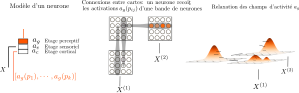
\includegraphics[width=\textwidth]{bijama_002.pdf}
    \caption{Exemple d'architecture construite avec le modèle Bijama~\parencite{menard05}.
    Chaque neurone d'une carte $i$ reçoit une entrée sensorielle $X\m{i}$ et des entrées corticales, indiquées figure de gauche.
    Dans cet exemple, deux cartes reçoivent des entrées sensorielles et corticales, et la troisième reçoit seulement des entrées corticales.
    Les activités corticales correspondent aux activités globales $a_g(p)$ des neurones situées dans une bande de même position dans la carte voisine, en gris dans la figure centrale. L'activité globale est une moyenne géométrique des activités sensorielles et corticales d'un neurone.
    Trois connexions sont représentées sur le schéma, mais tous les neurones reçoivent des connexions.
    La rétroaction entre les activités neuronales induit un phénomène dynamique de relaxation au sein de l'architecture, au cours duquel les entrées sensorielles restent inchangées et les activités globales des neurones évoluent vers un état limite stable. \label{fig:bijama}}
\end{figure}

Dans ce modèle présenté en figure~\ref{fig:bijama}, chaque neurone d'une carte est connecté via sa couche corticale à une rangée de neurones d'une carte modale. Cela revient donc à la transmission de champs d'activation entre cartes.
La mise à jour est asynchrone~: les connexions directes entre neurones génèrent la mise à jour des poids du neurone. Contrairement aux modèles précédemment présentés, l'activité prise en compte lors des connexions neuronales est l'activité globale du neurone. Le calcul de l'activité du neurone de la première carte dépend de l'activation des neurones de la deuxième, qui dépendent de l'activité de la première.
Les activités étant calculées de façon asynchrone, la présentation d'une entrée induit un processus dynamique de calcul d'activité au sein des neurones, au cours duquel les entrées thalamiques restent inchangées et les activités des neurones évoluent vers un état limite stable. Cette dynamique est appelée relaxation.
Cette activité finale est celle prise en compte par les neurones pour la mise à jour de leurs prototypes.

L'architecture SOMMA implémente également une architecture décentralisée pour de l'apprentissage multimodal (figure~\ref{fig:somma})
L'information transmise dans ce cas est une partie de l'activité des neurones, comme en Bijama. Comme dans ce modèle, les neurones sont structurés en étages, et l'étage cortical du neurone reçoit les activations des neurones situés dans une partie d'une autre carte.
Il s'agit ici de l'activité située dans un carré centré à la même position que le neurone courant, au lieu des bandes de Bijama.
L'information transmise entre cartes est ainsi également un champ d'activation. Les auteurs utilisent ici comme interface un champ d'activité réduit à une zone de la carte. Comme pour le modèle Bijama, SOMMA prend en compte les rétroactions dans le calcul d'activité de chaque carte, utilisant le même mécanisme de relaxation.


\begin{figure}
    \centering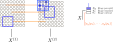
\includegraphics[width=0.9\textwidth]{SOMMA_002.pdf}
    \caption{
        Le modèle SOMMA \parencite{lefort_unlearning_2011,lefort_apprentissage_2012} associe les activités de différentes cartes, mais en réduisant les champs d'activité transmis aux neurones entourant le neurone situé en position courante. A gauche sont représentées les connexions entre les neurones de deux cartes, dans l'architecture SOMMA. \`A droite, le schéma d'un neurone d'une carte, comportant un étage sensoriel, cortical et global.
        Comme dans l'architecture Bijama, les rétroactions sont gérées par la dynamique de relaxation, laissant les champs d'activité évoluer vers un état stable.
    \label{fig:somma}}
\end{figure}

L'architecture proposée en \cite{baheux_towards_2014} cherche à transformer le modèle cellulaire de Bijama en s'appuyant sur des cartes auto-organisatrices classiques et l'applique au traitement de séquences. Cette architecture, décrite en figure~\ref{fig:baheux}, est composée de deux cartes. 
Chacune des cartes est composées de deux couches de poids $\w_e$ et $\w_c$. Une des cartes prend une entrée $\inpx_t$ correspondant à l'observation courante et relative à la couche de poids $\w_e$, comme une SOM classique. 
La deuxième couche de poids est relative à l'information contextuelle descendant de la seconde carte, qui est sa position du BMU $\bmu\m{1}$.
La seconde carte reçoit également deux entrées ~: l'entrée externe est la position du BMU $\bmu\m{1}(t-1)$ de l'état précédent et l'entrée contextuelle la position du BMU $\bmu\m{1}(t)$ de l'état courant. 
Chaque carte a ainsi des activations externes et contextuelles~: $a_e\m{1} = a_e\m{1}(p, \w_e\m{1},\inpx)$, $a_c\m{1} =  a_c\m{1}(p, \w_c\m{1},\bmu\m{2}_t)$, et $a_e\m{2} = a_e\m{2}(p, \w_e\m{2},\bmu\m{1}_{t-1})$, $a_c\m{2}(p, \w_c\m{2}, \bmu\m{1}_t)$.

Enfin, ces activations sont combinées dans chaque carte pour former une unique activité permettant de trouver le BMU~:
$$
a\m{i} = \sqrt{a_e\m{i}(\beta a_e\m{i} + (1-\beta) a_c\m{i})}
$$

Comme chaque carte reçoit en entrée la position de l'état courant du BMU de l'autre carte dépendant des boucles de rétroactions, le modèle laisse relaxer les activités en déplaçant petit à petit les BMUs de chaque carte, jusqu'à obtenir un état stable pour les activités. Cette relaxation est un parallèle dans une carte auto-organisatrice classique à la relaxation proposée en Bijama.
Cette position stable est utilisée pour déterminer le BMU final servant à la mise à jour des poids.
Ce modèle permet alors d'apprendre des séquences d'entrée. Alors qu'une carte simple différencierait les BMUs en fonction de la valeur de l'entrée, ce modèle génère une différenciation des BMUs en fonction de la position d'un élément dans la séquence.


\begin{figure}
    \centering
    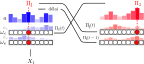
\includegraphics[width=0.7\textwidth]{baheux.pdf}
    \caption{Structures de deux cartes auto-organisatrices communicantes, \parencite{baheux_towards_2014}. Chaque carte est composée de trois couches d'activités, représentées séparément sur le schéma~: sur la première carte, une activité est relative à l'entrée $X$, l'observation. L'autre activité reçoit une entrée descendant de la seconde carte. Ces deux activités sont fusionnées en une activité globale servant à déterminer un BMU. La seconde carte reçoit ensuite deux entrées venant de la première carte~: le BMU de l'état courant et le BMU de l'état précédent. Un système de résonance est mis en place pour gérer les boucles de rétroactions entre BMUs, comme chaque carte reçoit le BMU de l'état courant de l'autre carte en entrée. Ce principe laisse évoluer dynamiquement les activités vers un état stable, utilisé ensuite pour la détermination du BMU final.\label{fig:baheux}}
\end{figure}


\subsubsection{Discussion}

Les architectures non hiérarchiques de cartes font donc apparaître deux grandes catégories~: les architectures centralisées, dans lesquelles une carte associative apprend à associer les activités de cartes sensorielles, et les architectures décentralisées.
Les architectures décentralisées apparaissent comme la version la plus pure d'une architecture modulaire~: lorsque les modules sont assemblés en architecture aucun rôle ne leur est attribué a priori, contrairement aux architectures centralisées faisant apparaître des cartes associatives sans entrées externes et des cartes modales. Dans ce cas, les modèles de connexions entre cartes sont différenciés.

La gestion des rétroactions entre cartes est un enjeu clé de la construction d'architectures décentralisées. Une première approche est de déconnecter, au sein d'une carte, l'apprentissage des poids liés aux entrées externes et des poids liés aux entrées contextuelles. Une carte a donc plusieurs BMUs, relatifs à une ou plusieurs couches de poids, et la mise à jour s'effectue couche par couche. Cette approche est celle privilégiée dans la plupart des travaux que nous avons relevés.
Les travaux menés dans notre équipe ont gardé la structure en couches ont fait le choix de ne pas séparer les activités des couches lors de l'apprentissage et de chercher un BMU commun.
La gestion des rétroactions est réalisée en introduisant un mécanisme de relaxation dans le calcul des activités. Dans les modèles cellulaires, l'architecture laisse les champs neuronaux dynamiques couplés évoluer, en tant que système dynamique, vers un état stable. Cette relaxation se traduit dans la version non-cellulaire par une boucle imbriquée au sein d'une itération, calculant le BMU par petits déplacements dans chaque carte, jusqu'à atteindre une position stable.
Nous choisissons dans cette thèse de privilégier cette seconde approche, introduisant un aspect de recherche dynamique du BMU dans les cartes. Un module n'a alors pas besoin de connaître des éléments de structure des autres modules~: il ne perçoit pas de différence entre un autre module qui aurait des entrées externes et un module qui n'aurait que des entrées  contextuelles.


\subsection{Apprentissage de séquences et architectures de cartes auto-organisatrices}

La capacité de traitement de séquences est une autre problématique d'utilisation des architectures de cartes. Nous avons également relevé des architectures cherchant à unir données spatiales et temporelles en un seul algorithme d'apprentissage. L'objectif d'un algorithme implémentant l'apprentissage de séquence est alors soit de prédire l'élément suivant d'une séquence de données, soit d'extraire des motifs temporels ou spatio-temporels se répétant dans les séquences de données d'entrée. 
La figure~\ref{fig:mouvement} illustre par exemple ce qu'on attend de l'apprentissage de séquences d'images d'un sportif~: en s'appuyant sur la succession des images présentées à l'algorithme, le but est d'extraire des catégories de mouvements comme \og tirer \fg{} ou \og marcher \fg{}, ce qui correspond à de la classification des séquences, ou de pouvoir compléter la vidéo en prédisant l'image suivante dans la séquence.
Ainsi, la création d'architectures pour le traitement de données multimodales se rapproche de la question du traitement de séquences. Rappelons également que l'enjeu de la multimodalité en robotique développementale inclue le traitement de données séquentielles.


Cette similarité entre données multimodales et séquentielles n'est pas seulement présente au niveau des objectifs d'application des architectures de cartes auto-organisatrices, mais bien dans la structure même du traitement des données. 
Une solution pour faire de l'apprentissage de séquences peut être de fournir en entrée d'un réseau non plus une donnée instantanée mais une suite de données, sous forme par exemple de fenêtre temporelle ou d'une représentation de la séquence.
Une autre solution est de prendre en compte l'état du réseau à l'instant précédent pour effectuer la mise à jour du réseau à l'état courant. 
Cette solution , implémentée dans de nombreux modèles d'apprentissage, se rapproche de la notion de transmission d'information entre modules d'une architecture, les modules étant ici les états de la carte à deux instants. Ces réseaux prenant en compte leur instant précédent pour calculer leur état actuel sont appelés réseaux récurrents ou récursifs.
Plusieurs modèles de cartes auto-organisatrices récurrentes, destinés à l'apprentissage de séquences, ont ainsi été proposés dans la littérature.

L'analyse des cartes récurrentes apparaît à la fois comme un enjeu de création d'une architecture générale de cartes auto-organisatrices dans la mesure où il s'agit de créer un modèle qui permet d'associer des modules et se laisse la possibilité d'y intégrer des connexions récurrentes au même titre qu'une connexion intercartes, et comme une source supplémentaire sur laquelle s'appuyer pour catégoriser les modes de transmission d'information entre cartes. Dans cette section, nous passons en revue différents modèles de cartes récurrentes et nous intéresserons aux modèles multi-cartes implémentant des connexions récurrentes au même titre que des connexions inter-cartes.

\begin{figure}
    \centering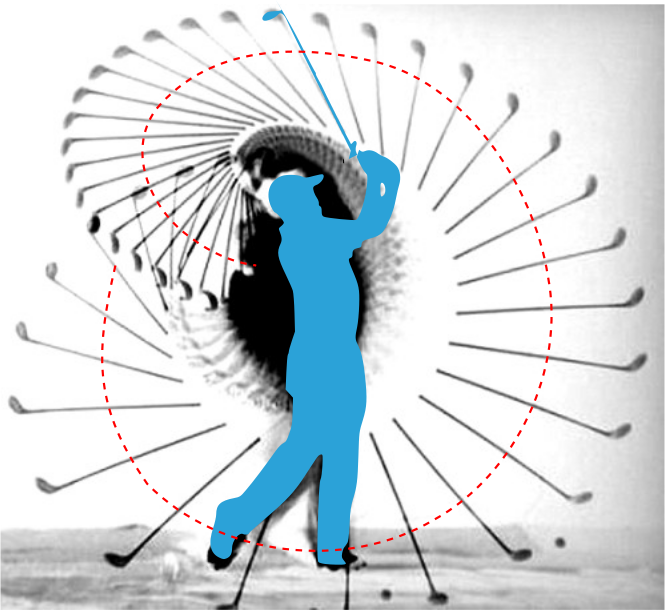
\includegraphics[width=0.6\textwidth]{movment_002.pdf}
    \caption{L'image présentée à un réseau (en bleu) correspond à un instant d'une séquence. L'objectif de l'apprentissage non supervisé de séquences est d'extraire une représentation d'une séquence d'entrée. Une utilisation commune est la classification de mouvements. La séquence "tirer" sera différente de la séquence "marcher".\label{fig:mouvement}}
 \end{figure}


\subsubsection{Cartes auto-organisatrices récurrentes}

Les modèles de cartes récurrentes existant dans la littérature s'appuient sur la transmission de représentation interne entre itérations. 
L'information transmise entre ces états rejoint les mécanismes relevés dans les architectures multi-cartes~: transmission du BMU en tant qu'entrée, transmission d'une activité, transmission du poids du BMU.

Parmi les premiers travaux autour des cartes auto-organisatrices, les cartes de Kohonen Temporelles TKM, dérivées ensuite en \emph{recurrent SOM} \cite{varsta_temporal_2001} utilisent l'activité $a$ d'une carte à l'instant précédent dans le calcul de l'activité à l'instant courant par un modèle d'intégrateur à fuite.

$$a(p,t) = (1-\alpha)a(p,t-1) + \alpha \dots (\inpx_t - \w_t(p))$$
Avec $\w(p)$ les poids de la carte et $\alpha \in [0,1]$ un coefficient de fuite.
$a$ correspond ici à une distance modifiée entre un prototype et l'entrée, et le BMU est alors calculé par $\Pi_t = \argmin_p(a(p,t)^2)$.
Le calcul de l'activité revient donc, au lieu de chercher la position dont le prototype $\w(p)$ est le plus proche de l'entrée $\inpx_t$, à chercher une position pour laquelle la distance entre le prototype et l'entrée est faible et pour laquelle la distance calculée par rapport aux entrées précédentes l'était aussi. Il s'agit d'un intégrateur à fuite dans la mesure ou l'influence de l'activité d'un instant sur les suivants décroit au cours du temps.

D'autres travaux reposent sur la transmission d'une information en tant qu'entrée, prise en compte dans le calcul de l'activité.
\`A chaque instant $t$, ces SOMs fusionnent deux entrées~: l'entrée venant de la séquence à apprendre, $X_t$ et l'entrée de contexte $\inpc_t$ interne à la carte.
Ainsi, les \emph{recursive SOMs} de \cite{Voegtlin2002RecursiveSM} utilisent en tant qu'entrée de contexte un vecteur contenant l'ensemble des activations des neurones de la carte à l'état précédent $\inpc_t = [a(t-1,p), p \in [0,N]^k]$ avec $k = 1, 2$ la dimension de la carte.
Les travaux de \cite{Buonamente2013SimulatingAW} proposent une version récurrente du modèle A-SOM présenté en section précédente. 
Le contexte considéré est alors également un ensemble d'activités de neurones. 
MSOM, proposée en \cite{Strickert2005MergeSF} s'appuie sur le poids du BMU. 
\`A chaque instant, l'entrée de contexte à transmettre à l'état suivant est définie comme une combinaison linéaire entre le poids du BMU courant et le contexte courant.
$$\inpc_t = \lambda \inpc_{t-1} + (1-\lambda)\w(\bmu_{t-1}) $$
Enfin, le modèle SOMSD, initialement proposé pour le traitement de données structurées \parencite{hagenbuchner_self-organizing_2003} puis étendu au traitement de séquences en \cite{hammer_recursive_2004,hammer_self-organizing_2005} réduit ce contexte à la position de la Best Matching Unit:
$$ \inpc_{t} = \bmu_{t-1}$$
Les mécanismes de transmission de contexte entre instants dans les cartes récurrentes s'appuient donc sur les mêmes mécanismes que ceux proposés dans le cadre d'architectures de cartes~: sélection de région de la carte, transmission d'activation, et enfin transmission du BMU.

\subsubsection{Architectures incluant des connexions temporelles}

Certains modèles s'appuient sur plusieurs cartes de Kohonen connectées, en y ajoutant une notion de traitement de séquences.
En \cite{parisiLL}, les auteurs développent une architecture de deux réseaux auto-organisés appelés \emph{grow when required networks} (GWR), voir figure \ref{fig:parisi}. Ces réseaux sont des versions incrémentales de cartes de Kohonen dans lesquelles des neurones sont ajoutés au cours de l'apprentissage, le processus de recherche de BMU restant ensuite similaire à une SOM classique.
Cette architecture utilise deux réseaux GWR pour apprendre des séquences, formant une mémoire épisodique et une mémoire sémantique.
La carte associée à la mémoire épisodique (G-EM) est une version récurrente du GWR, prenant en entrée courante $X_t$ et en entrée de contexte $\w(\Pi_{t-1})$, le poids du BMU à l'instant précédent.
La deuxième carte est une version classique du GWR. Elle prend en entrée le poids du BMU de la carte épisodique ainsi que la classe de la séquence courante, afin de mettre à jour ses poids.
Les auteurs utilisent leur architecture pour de la reconnaissance d'objets. Cependant, lors de l'apprentissage, les données ne sont pas présentées après un tirage aléatoire dans l'espace, mais sont présentées classe par classe~: tous les objets d'une même classe d'abord, etc. Les auteurs montrent que l'architecture est capable de bien prédire la classe d'un objet lors d'un test sur toutes les classes apprises. \`{A} titre de comparaison, une SOM classique apprendrait la classe du premier objet, puis l'oublierait pour se déplier entièrement sur la deuxième classe~; à terme, seule la dernière classe serait gardée en mémoire.
Ce type de structure prenant des entrées évoluant dans le temps et les gardant en mémoire s'inscrit dans l'apprentissage développemental. Nous entrevoyons ainsi l'intérêt que peuvent présenter des structures assemblant connexions temporelles et intercartes au sein d'une même architecture.
On ne peut pas vraiment parler d'architecture modulaire dans ces travaux, les deux couches de cartes étant différentes et spécialement conçues pour l'application d'apprentissage de séquence réalisée par les auteurs. Une logique de vérification externe aux cartes est par ailleurs utilisée pour ajouter ou non des neurones dans la couche supervisée. La carte récurrente est donc une manière de filtrer les entrées avant d'effectuer de l'apprentissage supervisé.
Par contre, la motivation de ce modèle est intéressante~: il s'agit cette fois de voir les deux cartes comme des modules d'apprentissage à différentes échelles temporelles. Avec les bonnes règles de mise à jour, cette propriété pourrait émerger dans des architectures modulaires.


Les travaux autour du modèle A-SOM mentionné précédemment ont également dérivé une version récurrente du modèle \parencite{Buonamente2015DiscriminatingAS} dans le but d'associer cartes récurrentes et multimodales en architecture.
Cette version récurrente est similaire à la version multi-cartes. Elle calcule alors son activité par rapport à son entrée et possède une seconde couche de poids qu'elle met à jour relativement au champ d'activation de l'instant précédent.
Cette structure est appliquée à la prédiction de mouvement. De la même façon qu'une architecture est capable, à partir d'une modalité, de prédire les valeurs correspondant à l'autre modalité, l'architecture incluant une version récurrente peut prédire la fin d'une séquence à partir de son début.
Nous n'avons cependant pas relevé de travaux les intégrant effectivement dans une architecture multi-cartes.

Enfin, nous pouvons revenir sur les travaux menés précédemment dans notre équipe décrits plus haut, qui proposent des architectures multi-cartes appliquées au traitement de séquence.
\cite{khouzam_neural_2014} utilise le modèle Bijama, permettant de construire des architectures de cartes auto-organisatrices cellulaires, dans un cadre de traitement de séquences.
Les connexions corticales des neurones d'une carte proviennent alors des activités des neurones de cette même carte au pas de temps précédent.
Le modèle à base de cartes auto-organisatrices classiques proposé en \cite{baheux_towards_2014} que nous avons décrit plus haut s'inscrit également dans un cadre de traitement de séquences. Le modèle montre qu'une carte de Kohonen au sein d'une architecture récurrente permet de différencier les BMUs d'une carte non seulement en fonction de la valeur de l'entrée mais également en fonction de la position dans la séquence. Ces résultats sont similaires à ce qu'on obtient avec une carte récurrente s'appuyant sur la transmission du BMU, sans relaxation, décrite par exemple en \cite{fix20}. La transformation du modèle récurrent en modèle multi-cartes montre la similarité existant entre récurrence et multimodalité et la possibilité d'inclusion de connexions récurrentes au sein d'un modèle multi-cartes.


\begin{figure}
    \centering
    \includegraphics[width=0.8\textwidth]{GWR.pdf}
    \caption{Architecture \emph{à double mémoire} proposée en \cite{parisiLL}. 
    La couche de mémoire épisodique, permettant la différenciation de séquences, prend en entrée externe un instant de la séquence d'entrée $X$ et en entrée de contexte le poids du BMU de l'instant précédent.
    La couche de mémoire sémantique est entraînée à partir du poids des BMU de la couche épisodique. Les auteurs ajoutent des conditions de classification supervisant la mise à jour de ces cartes, que nous ne détaillons pas sur ce schéma. Ce modèle est un exemple d'architecture assemblant cartes récurrentes et cartes classiques~; il s'agit ici d'un modèle semi-supervisé. Les auteurs utilisent cette architecture dans le cadre de l'apprentissage à long-terme.\label{fig:parisi}}
\end{figure}


\section{Discussion et axe de recherche}

La littérature portant sur les architectures de SOMs se divise donc en deux grandes catégories. D'une part, des travaux ont exploré des architectures hiérarchiques ou multicouches, se plaçant dans une optique d'amélioration des performances d'une SOM sur des applications de quantification vectorielle et de classification. Ces travaux relèvent du domaine de l'apprentissage automatique. 
Dans certains travaux, l'assemblage des cartes est régi par une surcouche algorithmique globale, ce qui nous amène à ne pas les considérer comme modulaires. 
D'autres travaux gèrent au contraire les connexions entre cartes à l'échelle d'une carte. Une carte prend alors le rôle de module d'une architecture. Chaque carte évolue alors uniquement grâce aux règles d'évolution internes qui ont été définies et grâce aux interfaces venant d'autres modules. Cependant, des conditions sur la structure hiérarchique de l'architecture sont préétablies.

D'autre part, certains travaux portent sur la création d'architectures comportant des rétroactions, que nous appelons architectures non hiérarchiques. Ces architectures non~hiérarchiques apportent moins de précondition de structure.
Ces travaux se placent plutôt dans le domaine des neurosciences computationnelles ou de la robotique. La création de ces architectures est en effet motivée par des considérations biologiques, les neurosciences suggérant que les aires du cerveau présentent des connexions rétroactives. 
Ces architectures à rétroactions permettent l'activation d'une carte par une autre et apportent aux SOMs une capacité de prise de décision et de prédiction lorsqu'elles sont au sein d'une architecture. Ces architectures non hiérarchiques se présentent soit sous la forme d'une architecture centralisée, dans laquelle une carte associative permet d'associer des cartes sensorielles, ou sous la forme d'une architecture décentralisée. 
Ce dernier cas est la forme la plus générique d'architecture modulaire de cartes de Kohonen~: la carte est un module autonome que l'on peut ajouter à une architecture existante sans différencier les modules a priori en fonction de leur position dans l'architecture.
Les modèles de cartes récurrentes, adaptées au traitement de séquence, se rapprochent par ailleurs des architectures multi-cartes par leur structure s'appuyant sur une transmission d'information, cette fois entre une même carte à deux pas de temps. 
Une architecture modulaire générique de cartes doit ainsi laisser la possibilité d'intégrer de façon indifférenciée des connexions classiques ou récurrentes au sein d'une architecture, dans une motivation d'apprentissage développemental.
Le tableau \ref{tab:bib} présente ainsi une comparaison des structures des principales architectures modulaires et récurrentes que nous avons relevées au cours de cette revue. 

\begin{table}[t!]
    \renewcommand{\arraystretch}{1.5}
    \caption{Comparaison des principaux modèles d'architectures relevés dans ce chapitre. Nous n'y faisons pas figurer les architectures sélectives, étant non modulaires. Les modèles très similaires sont regroupées sur une seule ligne. Les cartes récurrentes ne sont pas concernées par la question de séquence de mise à jour. \label{tab:bib}}
    \vspace{5mm}
    \begin{tabular}{p{2cm}p{6cm}p{2cm}p{5cm}}
        Modèle& Type& Mise à jour& Mode de transmission   \\
        \hline
        HSOM\footnotemark[1]& Hiérarchique & Séquentielle & Position du BMU  \\
        Deep SOM\footnotemark[2] & Hiérarchique & Séquentielle & Position du BMU   \\
        Autres \footnotemark[3] & Hiérarchique & Séquentielle & Poids du BMU \\
        \hline
        MMCM \footnotemark[4] & non hiérarchique, Centralisée & Séquentielle    & Positions BMU    \\                  
        SOIMA\footnotemark[5] & non hiérarchique, Centralisée & Séquentielle    & Champ d'activité \\
        Bijama\footnotemark[6] & non hiérarchique, Décentralisée &   Asynchrone    & Champ d'activité partiel \\ 
        A-SOM  \footnotemark[7] & non hiérarchique, Décentralisée       & Synchrone       & Champ d'activité \\
        SOMMA  \footnotemark[8]          & non hiérarchique, Décentralisée       & Synchrone       & Champ d'activité partiel \\
        \cite{jayaratne_bio-inspired_2018}           & non hiérarchique, Décentralisée       & Séquentielle    & Champ d'activité \\
        \cite{khacef_brain-inspired_2020}            & non hiérarchique, Décentralisée       & Séquentielle    & Champ d'activité \\
        \hline
        RSOM  \footnotemark[9]      & Récurrente                            &                & Champ d'activité \\
        MSOM   \footnotemark[10]& Récurrente                                   &                & Poids du BMU\\
        A-SOM   \footnotemark[11]& Récurrente                            &                & Champ d'activité\\
        Recursive SOM \footnotemark[12]& Récurrente                            &                & Champ d'activité\\
        SOMSD       \footnotemark[13]& Récurrente                       &               & Position du BMU \\
        \hline
        \cite{parisiLL} & Récurrente, Hiérarchique & Synchrone  & Poids du BMU \\
        \cite{baheux_towards_2014} & Récurrente, non hiérarchique & Synchrone & Position du BMU \\
    \end{tabular}
    \begin{tabular}{p{0.5\linewidth}p{0.5\linewidth}}
    \begin{itemize}\footnotesize
        \item[1]\cite{lampinen_clustering_1992,hagenauer_hierarchical_2013}\cite{Paplinski2005MultimodalFS}
        \item[2] \cite{liu_deep_2015},\cite{wickramasinghe_deep_2019}
        \item[4] \cite{dominey13}
        \item[3] \cite{dozono_convolutional_2016,mici_self-organizing_2018,nawaratne_hierarchical_2020-1,aly_deep_2020,wang_comparisonal_2007, gunes_kayacik_hierarchical_2007,luttrell_hierarchical_1989}
        \item[5] \cite{escobar-juarez_self-organized_2016}
        \item[6] \cite{menard05,khouzam_2013}
        \item[7]  \cite{johnsson_associating_2008}
    \end{itemize} & 
    \begin{itemize}\footnotesize
        \item[8] \cite{lefort_unlearning_2011}
        \item[9] \cite{varsta_temporal_2001}
        \item[10] \cite{Strickert2005MergeSF}
        \item[11] \cite{Buonamente2013SimulatingAW}
        \item[12] \cite{Voegtlin2002RecursiveSM}
        \item[13] \cite{hammer_self-organizing_2005}
    \end{itemize}
\end{tabular}
\end{table}

Nous avons remarqué que seulement peu de travaux ont exploré l'idée d'associer des SOMs en architectures non hiérarchiques.
Parmi ces quelques travaux, les interfaces entre cartes considérées par leurs auteurs s'appuient principalement sur la transmission de champs d'activation neuronaux.
La transmission de la position du BMU comme information entre cartes apparait au contraire comme un paradigme principalement utilisé dans le domaine des cartes hiérarchiques ainsi que certains modèles récurrents.
Ce mode de transmission exploite pleinement l'aspect topologique de la carte de Kohonen, est indépendante du type d'entrée fourni à une carte et est une valeur de faible dimension, donc intéressante pour le calcul. Ce paradigme permet aux architectures s'y appuyant de réaliser de bonnes performances en terme d'apprentissage automatique.
Seuls les travaux de \cite{dominey13} s'appuient sur transmission de la position du BMU dans le cadre des SOMs non hiérarchiques.
Les architectures décentralisées principalement proposées sous le prisme d'une inspiration biologique, ce qui justifie l'utilisation privilégiée de transmission d'activité~: les neurones biologiques sont connectés par des connexions neurones à neurones et se transmettent une activation. 
Or, le concept de BMU et de processus \emph{Winner Take All} intervenant dans une carte auto-organisatrice permet en fait de remplacer les champs neuronaux, proches de la biologie mais difficiles à paramétrer~\parencite{fix:hal-00869726} par un mécanisme global à la carte. Ce mécanisme s'éloigne de la plausibilité biologique mais permet des calculs plus rapides dans une SOM, tout en conservant les propriétés d'auto-organisation d'une carte. La transmission du BMU entre cartes au lieu d'activités apparaît donc comme un pendant plus computationnel de la transmission d'activité.

Le travail de recherche proposé dans cette thèse consiste à construire et étudier un modèle d'architecture de cartes bio-inspiré.
Nous cherchons à nous placer plutôt du côté du calcul informatique, laissant la biologie comme une inspiration et non en cherchant à la modéliser. 
Par cette inspiration biologique, il nous apparaît pertinent d'explorer la construction d'architectures non hiérarchiques décentralisées de cartes de Kohonen. Pour ses avantages en termes de coût de transmission et d'homogénéité des calculs, nous nous tournerons vers la transmission de la position du BMU comme information entre modules.
La plupart des architectures relevées dans la littérature s'appuient sur des mises à jour séquentielles. 
Une architecture générale incluant le traitement de séquences doit nécessairement gérer ses mises à jour de façon synchrone~; aussi nous choisirons de diriger nos recherches dans ce sens.
Nous proposerons donc une architecture non hiérarchique décentralisée de cartes de Kohonen, dont les mises à jour se font de façon synchrone. Les travaux que nous avons réalisés portent sur la définition et l'analyse des comportements générés par un tel modèle.
Nos travaux font suite aux travaux amorcés en \cite{baheux_towards_2014} sur des architectures récurrentes multimodales utilisant la transmission de la position du BMU entre des cartes de Kohonen et utilisant un mécanisme de relaxation pour gérer les rétroactions entre cartes.
Ces travaux exploitent des connexions intercartes mais restent appliqués au traitement de séquences.
Nous explorerons donc la construction d'architectures multi-cartes et continuerons le développement de ce modèle mais dans un cadre multimodal, afin de comprendre d'autres mécanismes intervenant dans une telle architecture.
Par leur motivation, qui est le développement d'un système multi-cartes générique, nos travaux se rapprochent aussi des travaux conduits sur l'architecture A-SOM~\cite{johnsson_associating_2008, johnsson_associative_2009,gil_sarasom_2015, Buonamente2015DiscriminatingAS}~; les choix de modèle sont cependant différents.

Nous dirigerons les travaux de cette thèse vers le traitement de données multimodales dans de petites architectures de deux et trois cartes.
Le but de cette thèse est d'identifier et de formaliser les comportements d'apprentissage générés par une petite structure non hiérarchique et de développer une méthode expérimentale et des représentations adaptées du modèle, dans une optique de création d'architecture comportant de nombreuses cartes.

\begin{figure*}[b]
    \centering\includegraphics[width=0.5\textwidth]{lego2.jpg}
\end{figure*}

\ifSubfilesClassLoaded{
    \printbibliography
    %\externaldocument{../main.tex}   
}{}
\end{document}